\documentclass[oneside, 8pt]{amsart}
\usepackage{amscd, amsmath, amssymb, amsthm, amsfonts, amstext, verbatim, mathtools, xfrac, microtype, nameref, thmtools}
\usepackage[breaklinks=true,unicode]{hyperref}
\usepackage[hyperref=true, backend=biber, bibencoding=utf8, giveninits=true, citestyle=numeric-comp, sortlocale=en_US, url=false, doi=false, eprint=true, maxbibnames=4]{biblatex}
\usepackage[capitalize]{cleveref}
\usepackage[matrix,arrow,curve]{xy}
\usepackage{tikz}
\usepackage{enumitem}
\usepackage[notref,notcite]{showkeys}

\addbibresource{paper.bib}
\renewbibmacro*{volume+number+eid}{\ifentrytype{article}{\- \iffieldundef{volume}{}{Vol.~\printfield{volume},}\iffieldundef{number}{}{ No.~\printfield{number},}}}
\renewbibmacro{in:}{\ifentrytype{article}{}{\printtext{\bibstring{in}\intitlepunct}}}
\newbibmacro{string+doi}[1]{\iffieldundef{doi}{\iffieldundef{url}{#1}{\href{\thefield{url}}{#1}}}{\href{http://dx.doi.org/\thefield{doi}}{#1}}}
\DeclareFieldFormat[article, inproceedings, inbook, book, thesis]{title}{\usebibmacro{string+doi}{\mkbibquote{#1}}}
\renewcommand*{\bibfont}{\footnotesize}

\newtheorem{theorem}{Theorem}
\newtheorem*{theorem*}{Theorem}
\newtheorem{lemma}{Lemma}
\newtheorem{prop}[lemma]{Proposition}
\newtheorem{corollary}[lemma]{Corollary}
\theoremstyle{remark} 

\theoremstyle{definition}
\numberwithin{lemma}{section}
\numberwithin{prop}{section}
\numberwithin{corollary}{section}
\newtheorem{df}[lemma]{Definition} \Crefname{df}{Definition}{Definitions}
\newtheorem{example}[lemma]{Example} \Crefname{example}{Example}{Examples}
\newtheorem{rem}[lemma]{Remark}
\newtheorem{cond}[lemma]{Condition}


\newlist{proplist}{enumerate}{1} \setlist[proplist]{label=(\roman{proplisti}), ref=\thethm.(\roman{proplisti}),noitemsep} \Crefname{proplisti}{Proposition}{Propositions}
\newlist{lemlist}{enumerate}{1} \setlist[lemlist]{label=(\roman{lemlisti}), ref=\thelem.(\roman{lemlisti}),noitemsep} \Crefname{lemlisti}{Lemma}{Lemmas}

\DeclareMathOperator{\Ker}{Ker}
\DeclareMathOperator{\Img}{Im}
\DeclareMathOperator{\St}{St}
\DeclareMathOperator{\GG}{G}
\DeclareMathOperator{\E}{E}
\DeclareMathOperator{\HH}{H}
\DeclareMathOperator{\K}{K}
\DeclareMathOperator{\KO}{KO}
\DeclareMathOperator{\GW}{GW}
\DeclareMathOperator{\colim}{colim}
\newcommand{\inv}{^{-1}}

\newcommand{\XX}{\mathcal{X}}           % (subset of) Steinberg generators
\newcommand{\RR}[1]{\mathcal{R}_{#1}}   % Steinberg relations
\newcommand{\catname}[1]{{\normalfont\textbf{#1}}} %Category name

\newcommand{\ZZ}{\mathbb{Z}}
\newcommand{\rA}{\mathsf{A}}
\newcommand{\rB}{\mathsf{B}}
\newcommand{\rC}{\mathsf{C}}
\newcommand{\rD}{\mathsf{D}}
\newcommand{\rE}{\mathsf{E}}
\newcommand{\rF}{\mathsf{F}}
\newcommand{\rG}{\mathsf{G}}

\numberwithin{equation}{section}

\title{On the presentation of orthogonal groups over polynomial rings}
\keywords {Steinberg group, $K_2$-functor, Serre problem
 {\em Mathematical Subject Classification (2010):} 19C20}
\author{Andrei Lavrenov}
\address{Mathematisches Institut der Universit\"at M\"unchen, Theresienstr. 39, D-80333 M\"unchen}
\email{avlavrenov at gmail.com}

\author {Sergey Sinchuk}
\address{Chebyshev laboratory, St. Petersburg State University, St. Petersburg, Russia}
\email {sinchukss at gmail.com}
\date {\today}

\begin{document}
\maketitle
\section{Introduction}


\section{Preliminaries}
$\langle \alpha, \beta \rangle = (\alpha, \beta^\vee) = (\alpha, \frac{2\beta}{(\beta, \beta)})$
Our convention for Cartan matrices is 
$A_{ij} = \langle \alpha_i, \alpha_j \rangle = (\alpha_i, \alpha_j^\vee)$.

\subsection{Steinberg groups}
Let $\Phi$ be a reduced and irreducible root system of rank $\geq 2$ and $R$ be a commutative ring with $1$. Recall that in this case the \emph{Steinberg group} $\St(\Phi, R)$ can be defined by means of generators $x_{\alpha}(s)$ (where $\alpha\in\Phi, s\in R$) and relations:
\begin{align}
& \phantom{[}
x_\alpha(s) \cdot x_\alpha(t) = x_\alpha(s+t),\ \alpha\in\Phi,\ s,t\in R; \label{rel:add}\\
& [x_\alpha(s), x_\beta(t)] = \prod\limits_{i,j\in\mathbb{N}}
 x_{i\alpha + j\beta}\left(N_{\alpha,\beta ij}\, s^i t^j\right),\quad \alpha,\beta\in\Phi,\ \alpha\neq\pm\beta,\ s,t\in R. \label{rel:CCF}
\end{align}
The indices $i$, $j$ appearing in the right-hand side of the above relation range over
all positive natural numbers such that $i\alpha + j\beta\in\Phi$.
The constants $N_{\alpha \beta i j}$ appearing in the right-hand side of \eqref{rel:CCF} are integers equal to $\pm 1,\pm 2,\pm 3$, they are called the {\it structure constants} of the Chevalley group $G_{sc}(\Phi, R)$. Several different methods have been proposed for choosing signs of these constants, see e.\,g.~\cite{V00}, \cite[\S~9]{VP}.

Whenever we speak of the Steinberg group $\St(\Psi, R)$ parametrized by a root subsystem $\Psi \subset \Phi$ we imply that the choice of structure constants 
 for $\St(\Psi, R)$ is compatible with that for $\St(\Phi, R)$ (i.\,e. the obvious map between these groups induced $\Psi\subseteq \Phi$ is well-defined).

In this paper we will be mostly interested in the case when the Dynkin diagram of $\Phi$ is {\it simply-laced}, i.\,e. does not contain double bonds. In this case the defining relations of $\St(\Phi, R)$ have the following simpler form:
\begin{align}
&x_{\alpha}(a)\cdot x_{\alpha}(b)=x_{\alpha}(a+b), \tag{R1}\\
&[x_{\alpha}(a),\,x_{\beta}(b)]=x_{\alpha+\beta}(N_{\alpha\beta} \cdot ab),\text{ for }\alpha+\beta\in\Phi, \tag{R2} \\
&[x_{\alpha}(a),\,x_{\beta}(b)]=1,\text{ for }\alpha+\beta\not\in\Phi\cup0. \tag{R3}
\end{align}
In the above formulae $a, b \in R$ and the integers $N_{\alpha, \beta} = N_{\alpha, \beta, 1, 1} = \pm 1$ are the structure constants of the Lie algebra of type $\Phi$. Although there is still some degree of freedom in their choice, these constants always must satisfy the relations, provided by the following lemma (cf.~\cite[\S~14]{VP}).
\begin{lemma} Suppose $\Phi$ is simply laced and $\alpha, \beta$ are roots of $\Phi$ such that $\alpha+\beta\in \Phi$, then holds
\begin{equation} \label{eq:simplest} N_{\alpha, \beta} = -N_{\beta,\alpha} = - N_{-\alpha, -\beta} = N_{\beta, -\alpha-\beta} = N_{-\alpha-\beta, \alpha}. \end{equation}
If, moreover, $\gamma \in \Phi$ is such that $\alpha,\beta,\gamma$ form a basis of a root subsystem of type $\rA_3$ then holds
\begin{equation} \label{eq:cocycle} N_{\beta,\gamma} \cdot N_{\alpha, \beta+\gamma} = N_{\alpha+\beta, \gamma} \cdot N_{\alpha, \beta}. \end{equation} \end{lemma}
In the computations below we use identities~\eqref{eq:simplest} without explicit reference.

For $\alpha\in\Phi$ and $s \in R^\times$ we define certain elements $w_\alpha(s), h_\alpha(s)$ of $\St(\Phi, R)$ (the latter ones are sometimes called {\it semisimple root elements}):
\begin{align*} w_\alpha(s) & =  x_\alpha(s) \cdot x_{-\alpha}(-s^{-1}) \cdot x_\alpha(s), \\ h_\alpha(s) & =  w_\alpha(s) \cdot w_\alpha(-1).  \end{align*}

Recall from~\cite[Lemma~5.2]{Ma69} that the following relations hold for semisimple root elements:
\begin{align} \label{eq:conj-h-x} {}^{h_\alpha(t)}\!x_\beta(u) & = x_\beta(t^{\langle \beta,  \alpha \rangle}u), \\ \label{eq:conj-h-h} {}^{h_\alpha(t)}\!h_\beta(u) & = h_\beta(t^{\langle \beta, \alpha \rangle} \cdot u) \cdot h_\beta(t^{\langle \beta,  \alpha \rangle})^{-1}. \end{align}

\subsection{\texorpdfstring{$\K_2$}{K2}-groups and symbols} In our computations we use two families of explicit elements of $\K_2(\Phi, R)$ called {\it Steinberg and Dennis--Stein symbols}. Notice that our treatment of symbols follows~\cite{DS73}. Recall that Steinberg symbols are defined for arbitrary $s, t \in R^\times$ as follows:
\begin{equation} \label{eq:steinberg} \{ s, t \}_\alpha = h_\alpha(st) \cdot h_\alpha^{-1}(s) \cdot h_\alpha^{-1}(t). \end{equation}
In turn, Dennis--Stein symbols are defined for arbitrary $a, b\in R$ satisfying $1 + ab \in R^\times$:
\begin{equation} \label{eq:dennis-stein}  \langle a,b \rangle _ \alpha = x_{-\alpha}\left(\tfrac{- b}{1 + ab}\right) \cdot x_{\alpha}(a) \cdot x_{-\alpha}(b) \cdot x_{\alpha}\left(\tfrac{- a}{1+ab}\right) \cdot h_{\alpha}^{-1}(1 + ab). \end{equation} 
Dennis--Stein symbol $\langle a, b \rangle_\alpha$ can be expressed through Steinberg symbols in the special case when either $a$ or $b$ is an invertible element of $R$. More specifically, the following formulae hold (cf.~\cite[p.~250]{DS73}).
\begin{equation} \label{DS-S-relationship} \langle a, b \rangle_\alpha = \{-a, 1+ab\}_\alpha\text{ for } a, 1+ab\in R^\times,\ \
 \{ s, t \}_\alpha = \left\langle -s, \tfrac{1 - t}{s} \right\rangle_\alpha\text{ for } s, t\in R^\times. \end{equation}
%Using~\eqref{eq:conj-h-h} it is easy to verify that \[[h_\alpha(s), h_\beta(t)] = \{s, t^{\langle \alpha, \beta \rangle}\}_\alpha = \{t, s^{\langle \beta, \alpha \rangle}\}_\beta^{-1}.\] 
Steinberg and Dennis--Stein symbols depend only on the length of $\alpha$, in particular they do not depend on $\alpha$ if $\Phi$ is simply-laced. If $\Phi$ happens to be {\it nonsymplectic}, i.\,e. $\Phi \neq \rA_1, \rB_2, \rC_{\geq 3}$, Steinberg symbols are antisymmetric and bimultiplicative, i.\,e. they satisfy the following identities: \begin{equation} \label{eq:symbol-properties} \{ u, st \} = \{ u, s\} \{ u, t \}, \ \{ u, v \} = \{ v, u\}^{-1}. \end{equation}
For these and other properties of symbols we refer the reader to~\cite{DS73}.

\begin{comment}
Suppose for a moment that $\langle \alpha, \beta \rangle = -1$ and  $\langle \beta, \alpha \rangle = -1$ then
\[ \{s, t^{-1} \} = \{s,  t^{-1}\}_\alpha = \{t, s^{-1} \}_\beta^{-1} = \{s^{-1}, t\} \]
In particular, $\{s, s^{-1}\} = \{s, s^{-1}\}^{-1}$ 
\end{comment}
The classical Matsumoto theorem (see~\cite[Theorem~5.10]{Ma69}) allows one to compute the group $\K_2(\Phi, R)$ in the special case when $R=k$ is a field. More concretely, it asserts that $\K_2(\Phi, k) \cong \K_2^\mathrm{MW}(k)$ provided $\Phi$ is symplectic and  $\K_2(\Phi, k) \cong \K_2^\mathrm{M}(k)$ otherwise. In the following lemma we 
recall the computation of the group $\K_2(\Phi, R)$ in the case $R=k[X, X\inv]$.
\begin{lemma}\label{K2-laurent-field} Let $\Phi$ be a reduced irreducible root system of type $\neq \rG_2$ and $k$ be arbitrary field. Then there is a split exact sequence of abelian groups
\[ \xymatrix{ 0 \ar[r] & \K_2(\Phi, k) \ar[r] & \K_2(\Phi, k[X, X^{-1}]) \ar[r] & H(\Phi, k) \ar[r] & 0,}\text{ in which} \]
\[ H(\Phi, k) = \left\{\begin{array}{ll} \K_1^\mathrm{MW}(k)& \text{if $\Phi$ is symplectic,}\\ k^* & \text{otherwise.}  \end{array}\right. \]  \end{lemma}
\begin{proof} Let us first consider the case of nonsymplectic $\Phi$, in which one can find a long root $\alpha\in \Phi$ in such a way that there is a commutative diagram of abelian groups
\[\xymatrixcolsep{5pc}\xymatrix{k^* \ar[r]^-{h} \ar[rrd]_{\{-, X\}} & \K_2(\Phi, k[X, X^{-1}]) \ar[r] & \K_2(\Phi, k(X)) \ar[d]^{\cong} \\
                                                                                      &                                 & \K_2^\mathrm{M}(k(X)),} \]
in which $h = \{ -, X \}_{\alpha}$ and the vertical map is an isomorphism by Matsumoto theorem.
Notice that the diagonal map is split by the obvious residue homomorphism and therefore is injective. This, in turn, implies that $h$ is also injective.
The assertion of the lemma now follows from~\cite[Satz~3]{Hur77} which asserts that for a nonsymplectic $\Phi$ holds $\K_2(\Phi, k[X, X\inv]) = \mathrm{Im}(h) \oplus \K_2(\Phi, k)$.

Consider now the case when $\Phi$ is symplectic. In this case the assertion of the lemma is just a reformulation of~\cite[Theorem~B]{MR91},
which asserts that for $\ell \geq 1$ one has $\K_2(\rC_\ell, k[X, X\inv] \cong \K_2(\rC_\ell, k) \oplus P(k)$, where
$P(k)$ is the set $k^* \times I_2(k)$ with the group structure given by
\[ (u, y) \cdot (v, z) = (uv, y + z - \langle\langle u, v\rangle\rangle).\]
Here $I^2(k)$ stands for the second power of the fundamental ideal $I(k)$ in the Witt ring $W(k)$ of $k$.
Recall that $\K_1^\mathrm{MW}(k)$ is isomorphic to the pullback of the diagram:
\[ \xymatrix{ \K_1^\mathrm{MW}(k) \ar[r] \ar[d] & I(k) \ar[d] \\ \K_1(k) \ar[r] & I(k)/I^2(k), } \]
in other words, it consists of pairs $[u, x]$ such that $x - \langle \langle u \rangle \rangle \in I^2(k)$.
It is easy to verify that the map $[u, x] \mapsto (u, \langle\langle u \rangle\rangle - x)$ defines an isomorphism of $\K_1^\mathrm{MW}(k)$ and $P(k)$. \end{proof}
 
\begin{corollary} \label{field-injectivity} For $\Phi\neq\rG_2$ the map $\St(\Phi, k[X]) \to \St(\Phi, k[X, X^{-1}])$ is injective. \end{corollary}
\begin{proof} Follows from consideration of the following commutative diagram:
\[\xymatrix{ & \K_2(\Phi, k) \ar[dl]_{\cong} \ar@{^{(}->}[dr] & \\
               \K_2(\Phi, k[X]) \ar[rr] &               & \K_2(\Phi, k[X, X^{-1}]),} \]
in which the left arrow is an isomorphism by the Korollar of~\cite[Satz~1]{Re75} and the right arrow is split injective by~\cref{K2-laurent-field}. \end{proof}

\subsection{Relative Steinberg groups and unstable K-groups} \label{sec:quillen}
In this subsection we recall the definitions and basic facts pertaining to relative Steinberg groups as defined by J.-L.~Loday in~\cite{Lo78}, where a theory of relative central extensions was developed and then applied to the stable Steinberg group $\St(R)$ from algebraic K-theory. The main goal of this subsection is to show that Loday's results can be applied to unstable Steinberg groups, and that the resulting relative groups enjoy many good properties of their stable counterparts.
Some of the results of this subsection have been briefly mentioned in~\cite{S15} (cf. e.\,g. Corollaries 3--4).

Recall that the category of (commutative) pairs $\catname{Pairs}$ is defined as follows.
Its objects are pairs $(R, I)$, in which $R$ is a commutative ring and $I$ is an ideal of $R$. A morphism of pairs $f \colon (R, I) \to (R', I')$ is, by definition, a ring map $f \colon R \to R'$ such that $f(I) \subseteq I'$. Notice that the mapping $(R, I) \mapsto (R \to R/I)$ defines a functor from $\catname{Pairs}$ the morphism category $\catname{CRings}^\rightarrow$.
If a pair $(R, I)$ is such that $R$ is a local ring with maximal ideal $I$, we call such a pair a {\it local pair}.

There is an obvious fully faithful embedding $\catname{CRings} \to \catname{Pairs}$ sending $R$ to $(R, R)$. For a given functor $S \colon \catname{CRings} \to \catname{Groups}$ a {\it relativization} of $S$ is any functor $\widetilde{S} \colon \catname{Pairs} \to \catname{Groups}$ extending $S$ in the obvious sense. Relativization of a functor is not unique.

Recall that {\it the double ring} $D_{R, I}$ of a pair $(R, I)$ is, by definition, the pullback ring $R \times_{R/I} R$. In other words, it is the ring consisting of pairs of elements of $R$ congruent modulo $I$. Denote by $p_0, p_1, \Delta$ the two obvious projections and the diagonal map $\xymatrix{D_{R,I} \ar@<1pt>[r] \ar@<-2.5pt>[r] & \ar@<-4pt>[l] R}$. It is clear that $p_0 \Delta = p_1 \Delta = id_{R}$.

Let $S \colon \catname{CRings} \to \catname{Groups}$ be a functor. Set $G_i = \Ker(S(p_i))$ and define {\it Loday's relativization} $S(R, I)$ as $ G_0 / [G_0, G_1]$. The map $S(p_1)$ induces a natural transformation $S(R, I) \to S(R)$. We denote this map by $\mu = \mu_{R,I}$ and its kernel by $C_S(R, I)$: \begin{equation} \label{LodayRelativization} \xymatrix{ 1 \ar[r] & C_S(R, I) \ar[r] & S(R, I) \ar^{\mu}[r] & S(R) \ar[r] & S(R/I) \ar[r] & 1.} \end{equation}

\begin{df} By definition, the {\it relative Steinberg group} $\St(\Phi, R, I)$ is the result of application of Loday's relativization to the functor $\St(\Phi, -)$. Notice that $\St(\Phi, R, I)$ is not a subgroup of $\St(\Phi, R)$ but rather its central extension by the abelian group $C_{\St(\Phi, -)}(R, I)$. For shortness we rename the latter group to $C(\Phi, R, I)$. \end{df}

Our next goal is to obtain a homological interpretation of the group $C(\Phi, R, I)$.
For doing this we need to recall some additional notation and terminology.

First of all, recall that a {\it central extension} of a group $G$ is a surjective map $\widetilde{G} \to G$, whose kernel is contained in the center of $\widetilde{G}$. 
A morphism of central extensions is a group-theoretic map $\widetilde{G} \to \widetilde{G}'$ over $G$.
A central extension is said to be {\it universal} if it is an initial object of the category of central extensions of $G$.

Recall that a {\it crossed module} is a triple $(M, N, \mu)$ consisting of a group $N$ acting on itself by left conjugation, an $N$-group $M$ and a map
 $\mu \colon M\to N$ of $N$-groups satisfying {\it Peiffer identity} $\mu(m) \cdot m' = m m' m^{-1}$. It can be shown that the image of $\mu$ is always
  a normal subgroup of $N$ and that the kernel of $\mu$, which we denote by $L$, is always contained in the center of $M$. %TODO: There's a problem with the side of the action :(
 
Let $\nu \colon N \twoheadrightarrow Q$ be a surjective group-theoretic map.
A {\it relative central extension of $\nu$} is, by definition,
a crossed module $(M, N, \mu)$ such that the cokernel of $\mu$ is $\nu$:
\begin{equation} \label{RelativeCentralExtension}
 \xymatrix{ 1 \ar[r] & L \ar[r] & M \ar^{\mu}[r] & N \ar^{\nu}[r] & Q \ar[r] & 1} \end{equation}

A morphism $(M, \mu) \to (M', \mu')$ of two relative central extensions of $\nu$ is, by definition, an $N$-group homomorphism $f\colon M \to M'$ such that $\mu' f = \mu$. 
A relative central extension is said to be {\it universal} if it is an initial object of the category of relative central extensions of $\nu$. 

It turns out that the set  $Ext(Q, N; L)$  of isomorphism classes of relative central extensions of $\nu$ by an abelian group $L$ can be classified by means of a certain cohomological invariant called {\it characteristic class}. More precisely, \cite[Th{\'e}or{\`e}me~1]{Lo78} asserts that there is a well-defined bijection $\xi \colon Ext(Q, N; L) \to \HH^3(Q, N; L)$.
 
For the rest of this subsection $S \xrightarrow{\pi} P \subseteq G$ is a triple of group-valued functors on the category of commutative rings satisfying the following assumptions:
\begin{enumerate} [label=(A\arabic*)]
 \item \label{req:left-exact} $G(D_{R, I}) \cong G(R) \times_{G(R/I)} G(R)$.
 \item \label{req:coeq} For every pair $(R, I)$ the coequalizer of $S(p_0), S(p_1)$ is precisely $S(R) \to S(R/I)$.
 \item \label{req:subfunc} $P(R)$ is a perfect normal subgroup of $G(R)$.
 \item \label{req:uce} The map $ \pi_R \colon S(R) \to P(R)$ is a universal central extension for all $R$. In particular, $\HH_1(S(R), \ZZ) = \HH_2(S(R), \ZZ) = 0$.
\end{enumerate}

\begin{lemma}\label{lem:relativeH3}
 For every pair $(R, I)$ the map $\mu \colon S(R, I) \to S(R)$ is a universal relative central extension of $\nu \colon S(R) \to S(R/I)$. The group $C_S(R, I)$ is naturally isomorphic to the relative homology group $\HH_3(S(R), S(R/I), \ZZ)$.
\end{lemma}
\begin{proof}
The action of $S(R)$ on $S(D_{R, I})$ given by ${}^g h = S(\Delta)(g) \cdot h \cdot S(\Delta)(g)^{-1}$ induces an action of $S(R)$ on $S(R, I)$.
The map $\mu \colon S(R, I) \to S(R)$ from~\eqref{LodayRelativization} is an $S(R)$-map with respect to this action.
From~\ref{req:left-exact} and $\varphi(G_i) \subseteq \Ker(G(p_i))$ we obtain that 
$G_0 \cap G_1 \subseteq \Ker(\pi_{D_{R, I}})$ and therefore is a central subgroup of $S(D_{R,I})$ by~\ref{req:uce}. Thus, we have verified the assumptions of~\cite[Proposition~6]{Lo78} which asserts that the map $\mu$ is a universal relative central extension of the coequalizer $\nu = \mathrm{coeq}(d_0, d_1)$. Since $\nu$ coincides with $S(R) \to S(R/I)$ by~\ref{req:coeq}, we have completed the proof of the first assertion of the lemma.

Set $N = S(R)$, $Q = S(R/I)$, $C = \HH_3(Q, N; \ZZ)$. Recall from the proof of~\cite[Th{\'e}or{\`e}me~2]{Lo78} that to every relative central extension $(M, \mu)$ of $\nu$ with kernel $L$ one can associate a map of abelian groups $C \to L$. This map is obtained from the characteristic class $\xi(M, \mu)$ via the isomorphism $\HH^3(Q, N; L) \cong \mathrm{Hom}(C, L)$ of the universal coefficients theorem.

In the special case $M = S(R, I)$ this construction produces a map $C \to C_{S}(R, I)$ whose naturality in $(R, I)$ follows from~\cite[Proposition~3]{Lo78}. 
This map is an isomorphism by~\cite[Th{\'e}or{\`e}me~2]{Lo78}. \end{proof}

We retain our notation for the functors $S, P$ and $G$.
For $i\geq 1$ we define the unstable Quillen K-functors $\K_{i}^{G, P}$ via
\[ \K_i^{G,P}(R) = \pi_i(BG(R)^+_{P(R)}). \]
It is not hard to obtain the following concrete description of these functors in the cases $i=1,2,3$.
\begin{lemma}\label{lem:lowerKgroups} There are natural isomorphisms \begin{enumerate}
 \item $\K_1^{G,P}(R) \cong G(R) / P(R)$;
 \item $\K_2^{G,P}(R) \cong \Ker(S(R) \to G(R))$;
 \item $\K_3^{G,P}(R) \cong \HH_3(S(R), \ZZ).$ \end{enumerate} \end{lemma}
\begin{proof} The first claim is obvious, the second and the third claim follow from~\ref{req:subfunc} and~\ref{req:uce} using the standard properties of the plus-construction, see \cite[\S~IV.1]{Kbook}   (cf. Exercises~1.8--1.9 ibid.) \end{proof}

Now let us give the example of a triple $(G, P, S)$ playing a key role in the present paper.
We denote by $\mathrm{O}_{2n}(R)$ and $\mathrm{EO}_{2n}(R)$ the orthogonal group of rank $n$ over a ring $R$ and its elementary subgroup, respectively
 (see e.\,g.~\cite{Su82} for the definition of these groups).
Now set $G_n = \mathrm{O}_{2n}(-)$, $P_n = \mathrm{EO}_{2n}(R)$, $S_n = \St(\rD_n, -)$ and let $\pi$ be the obvious projection $S_n \to P_n$.

It is easy to see that functors $G_n$, $P_n$ and $S_n$ satisfy \ref{req:left-exact} and \ref{req:coeq}.
By~\cite{Su82} the requirement~\ref{req:subfunc} is also satisfied for $n \geq 3$.
Finally, from~\cite[Corollary~5.4]{St71} and~\cite[Theorem~1]{LS17} it follows that $S_n$ and $P_n$ satisfy~\ref{req:uce} for $n \geq 5$.
We write $\KO_i(2n, R)$ as a shorthand for $\K_i^{G_n, P_n}(R)$.
%Notice that $\K_2(\rD_n, R) \subset \mathrm{KO}_2(n, R)$.

\begin{comment}
In the above definition we could have replaced the group $\mathrm{O}_{2n}$ with a different isogeneous form of the orthogonal group, e.\,g. 
 we could have chosen $G_n = \mathrm{SO}_{2n}$ or $G_n = \mathrm{Spin}_{2n}$ and then have defined $P_n$ as its elementary subfunctor.
Of course, this would change the functors $\K_i(G_n, P_n, -)$ for $i=1,2$ however, as the proof of~\cref{characterization} suggests
 it would not change $\K_3(G_n, P_n, -)$.
\end{comment}

We conclude this subsection with the following stability result (see~\cite[Theorem~9.4]{Pa89}).
\begin{theorem*}[Panin] \label{lem:Panin-stability}
 Let $R$ be either a field, principal ideal domain or a Dedekind domain. Set $a = 1,2$ or $3$ in each of these three cases, respectively.
 Then the stability map $\KO_i(2n, R) \to \KO_i(2(n+1), R)$ is an epimorphism for $n \geq b$ 
 and an isomorphism for $n \geq b + 1$, where $b = \mathrm{max}(2i, a+i-1)$. \end{theorem*}

\section{Proof of the first part of the injectivity theorem} \label{firstPart}
We start this section by recalling basic notation and facts pertaining to hermitian K-theory.
First of all, recall that the stable orthogonal K-groups $\KO_i(R) = \KO_i(\infty, R)$ are precisely the hermitian K-groups ${}_{-1}\!L_i(R)$ introduced by Karoubi in~\cite{Ka80}. We will need yet another redesignation for these groups $\KO_i(R)$, which comes from the theory of {\it higher Grothendieck--Witt groups of schemes}.
Recall that this theory, developed by M.~Schlichting, is a modern broad generalization of the classical hermitian K-theory of rings developed in~\cite{Ka80}.
We refer the reader to~\cite[\S~2]{FRS12} and~\cite[\S~2]{AF17} for the introduction to it.

For our purposes it suffices to restrict attention to the affine case, in which we can consider Grothendieck--Witt groups $\GW_i^{[k]}(R)$ for $i \geq 1,\ [k] \in \ZZ/4\ZZ$
 simply as a shorthand for the following groups
\begin{equation*} \GW_i^{[k]}(R) = \left\{\begin{array}{ll} \KO_i(R), & k = 0 \\ U_i(R), & k = 1 \\ \mathrm{KSp}_i(R), & k = 2 \\ {}_{-1}\!U_i(R), & k = 3. \end{array}\right. \end{equation*}
The groups ${}_{\pm 1}\!U_i(R)$, $\mathrm{KSp}_i(R)$ are defined in~\cite{Ka80} and we will not use their definition. 
What we need from Grothendieck--Witt groups is the following result due to M.~Schlichting.
\begin{theorem*}[Bass Fundamental Theorem]\label{bass-ft} Suppose that $R$ is a regular ring such that $2 \in R^*$, 
then for any $i\geq 1$, $k\in \ZZ/4\ZZ$ there is a natural split exact sequence of abelian groups \[ \xymatrix{ 0 \ar[r] & \GW_i^{[k]}(R) \ar[r] & \GW_i^{[k]}(R[X, X^{-1}]) \ar[r]  & \GW_{i-1}^{[k-1]}(R) \ar[r] & 0.} \] \end{theorem*}
\begin{proof} This is a very special case of~\cite[Theorem~9.13]{Sch16} and the remark that follows it. \end{proof}
We will use the above theorem only in the special case $i=0$, in which it boils down to an earlier result of Hornbostel, see~\cite[Corollary~5.3]{Ho05}.

%If we denote the kernel of the natural transformation $\mu$ from the definition of $\St(\Phi, R, I)$ by $C(\Phi, R, I)$ we obtain a natural exact sequence:
%\begin{equation} \label{relSteinberg-def}  \xymatrix{ 1 \ar[r] & C(\Phi, R, I) \ar[r]^{j} & \St(\Phi, R, I) \ar[r]^{\mu} & \St(\Phi, R) \ar[r]^{\pi} & \St(\Phi, R/I) \ar[r] & 1.} \end{equation}
%The group $C(\Phi, R, I)$ is trivial when $I$ is a splitting ideal of $R$, i.\,e. when the canonical map $R \to R/I$ splits, see \cite[Lemma~8]{S15}.

For the rest of this section let us fix the following notation.
Let $A$ be arbitrary commutative local ring with maximal ideal $M$ and residue field $k$.
Denote by $B = B_{A, M}$ the subring $A[X^{-1}] + M[X]$ of the ring $R = A[X, X^{-1}]$ and
by $I$ the ideal $M[X, X^{-1}]$ of $B$ (it is clear that $I$ is also an ideal of $R$).

\begin{lemma} \label{lem:prop41}
Assume additionally that the residue field $k$ is of characteristic $\neq 2$.
Then the canonical map $f\colon C(\rD_\ell, B, I) \to C(\rD_\ell, R, I)$ is surjective for $\ell \geq 7$. \end{lemma}
\begin{proof}
%There is a natural exact sequence:
% \[ \xymatrix{\K_3(G, P, R) \ar[r] & \K_3(G, P, R/I) \ar@{->>}[r] & C_S(R, I).} \]
Writing the starting portion of the homology long exact sequence for the map $\St(\rD_\ell, R) \to \St(\rD_\ell, R/I)$ 
and using the isomorphisms of~\cref{lem:relativeH3} and~\cref{lem:lowerKgroups} we obtain the following commutative diagram:
\begin{equation*}\xymatrix{
 \KO_3(2\ell, B) \ar[r] \ar[d] & \KO_3(2\ell, k[X]) \ar[d]_{f'} \ar@{->>}[r] & \ar[d]_{f} C(\rD_\ell, B, I) \\
 \KO_3(2\ell, R) \ar[r]        & \KO_3(2\ell, k[X, X^{-1}]) \ar@{->>}[r]        & C(\rD_\ell, R, I).}\end{equation*}
In view of Panin stability theorem the map $f'$ is precisely the canonical map $\GW_3^{[0]}(k[X]) \to \GW_3^{[0]}(k[X, X^{-1}])$.
By Bass fundamental theorem $\GW_3^{[0]}(k[X, X^{-1}]) \cong \GW_3^{[0]}(k) \oplus \GW_2^{[3]}(k),$
but since the group $\GW_2^{[3]}(k)$ is trivial by~\cite[Lemma~2.2]{FRS12}, the map $f'$ (and hence $f$) is surjective.
\end{proof} 
 
We will also need the following property of relative Steinberg groups which is a special case of {\it ``Tulenbayev lifting property''} discussed in~\cite[\S~2]{LS17}.
\begin{lemma}\label{lem:lemma32} Let $\Phi$ be a simply-laced root system of rank $\geq 3$,
Consider the following commutative square of canonical maps.
\[ \xymatrix{
    \St(\Phi, B, I) \ar[r] \ar[d] & \St(\Phi, B) \ar[d] \\
    \St(\Phi, R, I) \ar[r] \ar@{-->}^t[ur] & \St(\Phi, R) } \]
Then there exists a diagonal map $t$ which makes the diagram commute.   
\end{lemma} 
\begin{proof}
 Notice that $R$ is isomorphic to the principal localisation of $B$ at $X$
  and that $I$ is uniquely $X$-divisible in the sense of~\cite[\S~4]{LS17}.
 Thus, in the special case $\Phi = \rA_3$ the assertion of the lemma follows from~\cite[Theorem~3]{LS17}.
 In the general case the assertion of the lemma is a corollary of amalgamation theorem~\cite[Theorem~9]{S15} 
  (see~\cite[\S~2]{LS17} for more details).
\end{proof}

\begin{theorem} \label{thm41}
Suppose that $2 \in A^*$. Then for $\ell \geq 7$ the canonical map $\St(\rD_\ell, B) \to \St(\rD_\ell, R)$ is injective.
\end{theorem}
\begin{proof}
 Consider the following commutative diagram with exact rows, in which the lifting $t$ is obtained from~\cref{lem:lemma32}:
\begin{equation*} \xymatrix{
 C(\rD_\ell, B, I) \ar[r]^{\lambda_B} \ar@{->>}[d]_{f} & \St(\rD_\ell, B, I) \ar[r]^{\mu_B} \ar[d]_{g} &
 \St(\rD_\ell, B) \ar[r]^{\nu_B} \ar[d]_{h} & \St(\rD_\ell, k[X]) \ar[d]_{i} \\
 C(\rD_\ell, R, I) \ar[r]^{\lambda_R}         & \St(\rD_\ell, R, I) \ar[r]^{\mu_R} \ar@{-->}[ur]^{t}&
 \St(\rD_\ell, R) \ar[r]^-{\nu_R}        & \St(\rD_\ell, k[X, X^{-1}]).
}\end{equation*}
Let $a$ be an element of $\Ker(h)$. Since $i$ is injective by~\cref{field-injectivity}, the element $a$
 also lies in $\Ker(\nu_B)$ and hence comes from some $b \in \St(\rD_\ell, B, I)$ via $\mu_B$.
Since $g(b) \in \Ker(\mu_R)$ there exists some $c \in C(\rD_\ell, R, I)$ such that $\lambda_R(c) = g(b)$. 
By~\cref{lem:prop41}, $f$ is surjective, therefore $c = f(d)$ for some $d \in C(\rD_\ell, R, I)$.
The required assertion now follows from the following computation:
 \[ 1 = \mu_B\lambda_B(d) = tg\lambda_B(d) = t\lambda_Rf(d) =t(g(b)) = \mu_B(b) = a. \qedhere \]
\end{proof}

\section{Elementary calculations in relative Steinberg groups}
\begin{comment}
Hall-Witt identity
\[ [[ y^{-1}, x], z] ^ {y^{-1}}  [[ z^{-1}, y], x] ^ {z^{-1}}  [[ x^{-1}, z], y] ^ {x^{-1}} = 1 \]
\[ [[ y^{-1}, x], z]  \cdot [[ z^{-1}, y], x] ^ {z^{-1}y} \cdot  [[ x^{-1}, z], y] ^ {x^{-1}y} = 1. \]
\[ [[ z^{-1}, y^{-1}], x] ^ {z^{-1}y^{-1}} \cdot  [[ x^{-1}, z], y^{-1}] ^ {x^{-1}y^{-1}} = [z, [ y, x]] . \]
\[  . \]
\end{comment}
Throughtout this let $\Phi$ is a simply laced root system, $R$ is a commutative ring, and $I, J$ are two its ideals. 
We denote by $\overline{\St}(\Phi, R, I)$ the kernel of the map $\St(\Phi, R) \to \St(\Phi, R/I)$.
This group coincides with the image in $\St(\Phi, R)$ of the relative group $\St(\Phi, R, I)$ defined in~\cref{sec:quillen}.

Denote by $\St(\Phi, I)$ the subgroup of $\St(\Phi, R)$ generated as a group by root unipotents of level $I$.
It is clear that $\overline{\St}(\Phi, R, I)$ contains $\St(\Phi, I)$ and, in fact, is its normal closure.
We also denote by $\overline{H}(\Phi, R, I)$ the subgroup of $\overline{\St}(\Phi, R, I)$ generated by the semisimple root elements $h_\alpha(u)$ and symbols $\{u, v\}$, $u \in (1+I)^\times$, $v \in R^\times$, $\alpha\in \Phi$.

We define the following two families of elements of $\overline{\St}(\Phi, R, I)$:
\begin{itemize}
 \item $z_\alpha(s, \xi) := x_\alpha(s)^{x_{-\alpha}(\xi)}$ defined for $\xi \in R$, $s \in I$;
 \item $c_\alpha(s, t) = [x_\alpha(s), x_{-\alpha}(t)]$ defined for $s \in I$, $t \in J$.
\end{itemize}

\begin{lemma}\label{Zrels} The elements $z_\alpha(s, \xi)$ satisfy the following relations for all $\xi, \eta\in R$, $s\in I$:
\begin{enumerate} 
\item\label{Z1} $z_{\alpha}(s, \xi) ^ {x_{-\alpha}(\eta)} = z_{\alpha}(s, \xi + \eta)$;
\item\label{Z2} $z_{\beta}(s, \xi) ^ {x_{\alpha}(\eta)} = x_{\alpha} (- s\xi \eta) \cdot x_{\alpha+\beta} (N_{\beta, \alpha}\cdot s\eta)     \cdot z_{\beta}(s, \xi)\ \text{if}\ \alpha + \beta \in \Phi$;
\item\label{Z3} $z_{\beta}(s, \xi) ^ {x_{\alpha}(\eta)} = x_{\alpha} (s\xi \eta) \cdot x_{\alpha-\beta} (N_{\beta,-\alpha}\cdot s\xi^2\eta) \cdot z_{\beta}(s, \xi)\ \text{if}\ \alpha - \beta \in \Phi$;

\item\label{Z4} $z_{\beta}(s, \xi) ^ {x_{\alpha}(\eta)} = z_{\beta}(s, \xi)\ \text{if}\ \alpha\perp\beta$;
\item\label{Z5} If $\alpha+\beta\in\Phi$, then holds:
\begin{multline} \nonumber z_{\alpha+\beta}(s\eta, \xi) = x_\alpha(\epsilon s)\cdot x_{-\beta}(-s\xi) \cdot x_{\beta}(s\xi\eta^2) \cdot x_{\alpha+\beta}(s \eta) \cdot \\ \cdot z_\alpha(-\epsilon s, -\epsilon \xi\eta) \cdot
  x_{-\alpha}(-\epsilon s\xi^2\eta^2) \cdot x_{-\alpha-\beta}(- s \xi^2 \eta) \cdot z_{-\beta}(s\xi, -\eta)\text{ where $\epsilon = N_{\alpha,\beta}$.}\end{multline}
\end{enumerate} \end{lemma}
\begin{proof}
The first four assertions are contained in~\cite[Lemma~9]{S15}, so it remains to verify the last assertion.
Direct computation shows that
\begin{multline} \nonumber
  z_{\alpha+\beta}(s\eta, \xi) = [x_\alpha(\epsilon s)^{x_{-\alpha-\beta}(\xi)}, x_\beta(\eta)^{x_{-\alpha-\beta}(\xi)}] =
  [x_\alpha(\epsilon s) x_{-\beta}(-s\xi), x_{\beta}(\eta) x_{-\alpha}(\epsilon \xi\eta)] = \\ 
  = x_\alpha(\epsilon s) \cdot x_{-\beta}(-s\xi) \cdot z_\alpha(-\epsilon s, -\epsilon \xi\eta)^{x_{\beta}(-\eta)} \cdot z_{-\beta}(s\xi, -\eta)^{x_{-\alpha}(-\epsilon \xi\eta)},
\end{multline} 
and the required assertion follows from~\eqref{Z2}.
\end{proof}

Let us mention an immediate application of the just proved lemma. 
First of all, recall the following two results in which two generating sets for the group $\overline{\St}(\Phi, R, I)$ are described.
\begin{theorem*}[Stein--Tits--Vaserstein]
 For arbitrary $\Phi$ of rank $\geq 2$ the group $\overline{\St}(\Phi, R, I)$ is generated by elements $z_\alpha(s, \xi)$, $\alpha \in \Phi$, $s \in I$, $\xi \in R$.
\end{theorem*} \begin{proof} See e.\,g.~\cite[Theorem 2]{Va86}. \end{proof}

For a subset of roots $U \subseteq \Phi$ we denote by $\mathcal{Z}(U, R, I)$ the subset of roots consisting of elements $x_\alpha(s)$, $s \in I$, $\alpha \in \Phi$ and $z_\alpha(s, \xi)$, $\alpha \in U$, $s\in I$, $\xi \in R$.

\begin{theorem*}[Stepanov] For arbitrary $\Phi$ of rank $\geq 2$ the group $\overline{\St}(\Phi, R, I)$ is generated as a group by the subset $\mathcal{Z}(\Sigma_S, R, I)$.
 Here $\Sigma_S$ denotes the special part of an arbitrary parabolic subset of roots $S \subseteq \Phi$.
\end{theorem*} \begin{proof} See~\cite[Lemma~4]{S15}. \end{proof}

\begin{rem} For a simply-laced $\Phi$ Stepanov's theorem can be deduced from Stein--Tits-Vaserstein theorem by means of~\cref{Zrels}. Indeed, consider the operator $d \colon 2^\Phi \to 2^\Phi$ of root subsets given by $d(U) = U \cup (U - U)\cap \Phi$, $U \subseteq \Phi$. In other words, $d$ adjoins to $U$ all differences of roots from $U$ which are themselves roots. It is not hard to show that for any parabolic subset $S \subseteq \Phi$ the subset $\Sigma_S$ has the property that $d^n(\Sigma_S) = \Phi$ (in fact, $n=2$). It remains to see that relation~\eqref{Z5} immediately implies that every group $G$ containing $\mathcal{Z}(U, R, I)$ also contains $\mathcal{Z}(dU, R, I)$. \end{rem}

We will need the following variant of Hall--Witt identity:
\begin{equation} \label{HW-variant} [[x, y], z] = \left([x^{-1}, [ y^{-1}, z]] ^ {y^{-1}} \cdot [y, [ z^{-1}, x^{-1}]] ^ {z^{-1}} \right)^{x^{-1}}.\end{equation}
\begin{lemma} \label{Crels}
The elements $c_\alpha(s, t)$ satisfy the following relations for all $s\in I,\ t\in J,\ \xi\in R$.
 \begin{enumerate}
 \item \label{C1} $[c_\beta(s, t), x_{\alpha}(\xi)] = x_{\alpha}(- st\xi) \cdot x_{\beta+\alpha}(N_{\alpha,\beta}s^2t\xi)$ if $\alpha+\beta \in \Phi$;
 \item \label{C2} $[c_\beta(s, t), x_{\alpha}(\xi)] = x_{\alpha}(st\xi + s^2t^2\xi) \cdot x_{\alpha-\beta}(N_{-\alpha, \beta}st^2\xi)$ if $\alpha-\beta \in \Phi$;  
 \item \label{C3} $[c_\beta(s, t), x_{\alpha}(\xi)] = 1$ if $\alpha \perp \beta$;  
 \item \label{C4} If $\alpha+\beta\in\Phi$ then holds:
  \[c_{\alpha+\beta}(s, t\xi) = [x_{\beta}(st), x_{-\beta}(\xi)] ^ {x_{\alpha+\beta}(-s) x_{-\alpha}(\epsilon t)} \cdot c_{\alpha}(\epsilon s\xi, -\epsilon t)^{-1} \cdot x_{-\beta}(-st\xi^2),\]
  where $\epsilon = N_{\alpha,\beta}$.
 \end{enumerate}
\end{lemma}
\begin{proof}
To verify~\eqref{C1} suppose $\alpha + \beta \in \Phi$ and compute
\begin{multline} \nonumber [c_{\beta}(s, t), x_{\alpha}(\xi)]  = [x_{\beta}(s), x_{-\beta}(t)] \cdot [x_{-\beta}(t), x_{\beta}(s)\cdot x_{\beta+\alpha}(N_{\alpha, \beta} \cdot s\xi)] = \\
 = {}^{x_\beta(s)}\![x_{-\beta}(t), x_{\alpha+\beta}(N_{\alpha, \beta} \cdot s\xi)] = x_{\alpha}(- st\xi) \cdot x_{\alpha+\beta}(N_{\alpha,\beta} \cdot s^2t\xi). \end{multline}

In the case $\alpha-\beta \in \Phi$ the second assertion directly follows from~\eqref{HW-variant}:
\begin{multline} \nonumber
[[x_\beta(s), x_{-\beta}(t)], x_{\alpha}(\xi)] = \\
= \left([x_\beta(-s), [ x_{-\beta}(-t), x_{\alpha}(\xi)]] ^ {x_{-\beta}(-t)} \cdot [x_{-\beta}(t), [ x_{\alpha}(-\xi), x_\beta(-s)]] ^ {x_{\alpha}(-\xi)}\right)^{x_\beta(-s)} = \\
= x_{\alpha}(-N_{\beta, \alpha-\beta} N_{\alpha,-\beta} \cdot s t \xi) ^ {x_{-\beta}(-t) \cdot x_\beta(-s)} = x_{\alpha}(s t \xi) ^ {x_{-\beta}(-t) \cdot x_\beta(-s)} = \\
= x_{\alpha}(st\xi) \cdot x_{\alpha-\beta}(-N_{\alpha,-\beta}\cdot st^2\xi)^{x_\beta(-s)} = x_{\alpha}(st\xi + s^2t^2 \xi) \cdot x_{\alpha-\beta}(N_{-\alpha,\beta}\cdot st^2\xi). \end{multline}

Finally, the final relation can be verified by the following direct computation, which involves identity $[x, yz]^y = [y^{-1}, x] \cdot [x, z]$ and \eqref{HW-variant} with both sides of the equation inverted:
\begin{multline} \nonumber [x_{\alpha+\beta}(s), x_{-\alpha-\beta}(t\xi)] = [x_{\alpha+\beta}(s), [x_{-\alpha}(-\epsilon t), x_{-\beta}(\xi)]] = \\ 
= \left([[ x_{\alpha+\beta}(-s), x_{-\alpha}(\epsilon t)], x_{-\beta}(\xi)] ^ {x_{\alpha+\beta}(-s)} \cdot  [[ x_{-\beta}(-\xi), x_{\alpha+\beta}(s)], x_{-\alpha}(\epsilon t)] ^ {x_{-\beta}(-\xi)}\right)^{x_{-\alpha}(\epsilon t)} = \\
= [x_{\beta}(st), x_{-\beta}(\xi)] ^ {x_{\alpha+\beta}(-s) x_{-\alpha}(\epsilon t)} \cdot  [ x_{\alpha}(\epsilon s\xi), x_{-\alpha}(\epsilon t)] ^ {x_{-\beta}(-\xi)x_{-\alpha}(\epsilon t)}  = \\
= [x_{\beta}(st), x_{-\beta}(\xi)] ^ {x_{\alpha+\beta}(-s) x_{-\alpha}(\epsilon t)} \cdot  [ x_{\alpha}(\epsilon s\xi), x_{-\alpha}(\epsilon t) x_{-\alpha-\beta}(t\xi)] ^ {x_{-\alpha}(\epsilon t)} = \\
= [x_{\beta}(st), x_{-\beta}(\xi)] ^ {x_{\alpha+\beta}(-s) x_{-\alpha}(\epsilon t)} \cdot  [x_{-\alpha}(-\epsilon t), x_{\alpha}(\epsilon s\xi)] \cdot [x_{\alpha}(\epsilon s\xi), x_{-\alpha-\beta}(t\xi)] = \\
= [x_{\beta}(st), x_{-\beta}(\xi)] ^ {x_{\alpha+\beta}(-s) x_{-\alpha}(\epsilon t)} \cdot c_{\alpha}(\epsilon s\xi, -\epsilon t)^{-1} \cdot x_{-\beta}(-st\xi^2). \qedhere
\end{multline}

\begin{comment}
\begin{multline} 
 [x_\alpha(m), x_{-\alpha}(X\xi)] = [x_\alpha(m), [x_{-\alpha-\beta}(N_{-\alpha-\beta, \beta} X), x_{\beta}(\xi)]] = \\ = \left([[ x_\alpha(m), x_{-\alpha-\beta}(-N_{-\alpha-\beta, \beta}X)], x_{\beta}(\xi)] ^ {x_\alpha(-m)} \cdot  [[ x_{\beta}(-\xi), x_\alpha(m)], x_{-\alpha-\beta}(-N_{-\alpha-\beta, \beta}X)] ^ {x_{\beta}(-\xi)}\right)^{x_{-\alpha-\beta}(-N_{-\alpha-\beta, \beta}X)} = \\ = \left([x_{-\beta}(-N_{-\alpha-\beta,\beta}N_{\alpha,-\alpha-\beta}mX), x_{\beta}(\xi)] ^ {x_\alpha(-m)} \cdot  [ x_{\alpha + \beta}(-N_{\beta, \alpha}m\xi), x_{-\alpha-\beta}(-N_{-\alpha-\beta, \beta}X)] ^ {x_{\beta}(-\xi)}\right)^{x_{-\alpha-\beta}(-N_{-\alpha-\beta, \beta}X)} =
\end{multline}
\end{comment}
\end{proof}

\subsection{Computation of the kernel of the map of evaluation at \texorpdfstring{$0$}{0}.}
For the rest of this subsection $A$ denotes a local ring with maximal ideal $M$.
The aim of this subsection is to describe a generating set for the kernel of the map $ev_{X=0}^*\colon\overline{\St}(\Phi, A[X], M[X]) \to \overline{\St}(\Phi, A, M)$
induced by the ring homomorphism of evaluation at $0$. Denote this kernel by $K(A[X], M[X])$.

It is obvious that $K(A[X], M[X])$ contains the subgroup $\overline{\St}(\Phi, A[X], XM[X])$.
It turns out that although being larger than this subgroup, $K(A[X], M[X])$ contains very few extra generators, which can all be explicitly described.

Since $ev_{X=0}^*$ admits a section, we can consider $\overline{\St}(\Phi, A, M)$ and $\St(\Phi, M)$ as subgroups of $\overline{\St}(\Phi, A[X], M[X])$,
 moreover, one has $\overline{\St}(\Phi, A[X], M[X]) = \overline{\St}(\Phi, A, M) \cdot K(A[X], M[X]).$
\begin{lemma} The following decomposition holds
 \[ K(A[X], M[X]) = \overline{\St}(\Phi, A[X], XM[X]) \cdot \left[\St(\Phi, XA[X]),\ \overline{\St}(\Phi, A, M)\right].\] \end{lemma}
\begin{proof} Fix $g \in K(A[X], M[X])$ and write it as $g(X) = \prod_i z_{\alpha_i}(f_i(X), \xi_i(X))$ for some $f_i(X) = f_i(0) + Xf_i'(X) \in M[X]$, $\xi_i(X) = \xi_i(0) + X\xi_i'(X) \in A[X]$.
 It is clear that modulo $\overline{\St}(\Phi, A[X], XM[X])$ the element $g(X)$ is congruent to $g_1(X) = \prod_i z_{\alpha_i}(f_i(0), \xi_i(X)).$ 
 
 Now each factor $z_{\alpha_i}(f_i(0), \xi_i(X))$ can be written as follows:
 \[z_{\alpha_i}(f_i(0), \xi_i(0))^{x_{-\alpha_i}(X\xi'_i(X))} = [x_{-\alpha_i}(-X\xi'_i(X)), z_{\alpha_i}(f_i(0), \xi_i(0))] \cdot z_{\alpha_i}(f_i(0), \xi_i(0)).\]
 Since the subgroup $C_0 = \left[\St(\Phi, XA[X]), \overline{\St}(\Phi, A, M)\right]$ is normalized by $\overline{\St}(\Phi, A, M)$ 
 (this follows e.\,g. from the formula $[g, h]^{h_1} = [h_1^{-1}, g][g, h_1^{-1}h]$) we conclude that $g_1(X)$ is congruent to $\prod_i z_{\alpha_i}(f_i(0), \xi_i(0)) = g(0) = 1$ modulo $C_0$,
 which implies the assertion. \qedhere \end{proof}

\begin{theorem*}[Stein] One has $\overline{\St}(\Phi, A, M) = U(\Phi^+, M) \cdot \overline{H}(\Phi, A, M) \cdot U(\Phi^-, M).$ \end{theorem*} \begin{proof} See~\cite[Theorem~2.4]{Ste73}. \end{proof}

\begin{prop} \label{Kgen} The subgroup $K(A[X], M[X])$ is generated as an abstract group by the subgroup $\overline{\St}(\Phi, A[X], XM[X])$ and
 the elements $[x_\alpha(m), x_{-\alpha}(X\xi)]$, $m \in M$, $\xi \in A[X]$, $\alpha \in \Phi$. \end{prop}
\begin{proof} Notice that it follows from~\eqref{eq:conj-h-x} $\overline{H}(\Phi, A, M)$ normalizes both $\St(\Phi, XA[X])$ and $\St(\Phi, M)$ and, moreover, that $[\overline{H}(\Phi, A, M),\ \St(\Phi, XA[X])] \subseteq \overline{\St}(\Phi, A[X], XM[X])$. 

Denote by $C_1$ the commutator subgroup $[\St(\Phi, XA[X]), \St(\Phi, M)]$.
It is clear that for $g \in \St(\Phi, XA[X])$, $h \in \overline{H}(\Phi, A, M)$, $u^+ \in U(\Phi^+, M)$, $u^- \in U(\Phi^-, M)$ holds:
\[ [g, h u^+ u^-] = [g, h] \cdot [{}^{h}\!g, {}^{h}\!(u^+u^-)] \in \St(\Phi, A[X], XM[X]) \cdot C_1.\]
Since $C_0$ is generated by the above commutators and $\overline{\St}(\Phi, A[X], XM[X])$ is a normal subgroup of $\St(\Phi, A[X])$
we obtain that $C_0 \subseteq \overline{\St}(\Phi, A[X], XM[X]) \cdot C_1$ and consequently that
$K(A[X], M[X]) = \overline{\St}(\Phi, A[X], XM[X]) \cdot C_1.$
 
It is clear that modulo $\overline{\St}(\Phi, A[X], XM[X])$ the commutator subgroup $C_1$ is generated by elements of the form $[x_\alpha(m), x_{-\alpha}(X\xi)]^g$, where $m \in M$, $\xi \in A[X]$, $g \in \St(\Phi, A[X])$.
Thus, it remains to show that commutators $[[x_\alpha(m), x_{-\alpha}(X\xi)], g]$ belong to $\overline{\St}(\Phi, A[X], XM[X])$.
Since the latter subgroup is normal it suffices to prove this inclusion in the special case when $g$ is a member of some generating set for $\St(\Phi, A[X])$.
Clearly, the set consisting of $x_\beta(\xi)$, $\xi \in A[X]$, $\beta \neq \pm \alpha$ is such a generating set, 
 and in this case the required inclusions follow from~\eqref{C1}--\eqref{C3} of~\cref{Crels}. \end{proof}

\begin{corollary} \label{Kgen-strong} For a local pair $(A, M)$ and arbitrary fixed root $\gamma$ of an irreducible simply-laced root system $\Phi$ the subgroup $K(A[X], M[X])$ is generated as a group by $\overline{\St}(\Phi, A[X], XM[X])$ and the elements $c_{\gamma}(m, X\eta)$, where $m \in M$, $\eta \in A[X]$. \end{corollary}
\begin{proof} Substituting $\xi = 1$, $s = m$, $t = X\eta$ into relation~\eqref{C4} of~\cref{Crels} we obtain that modulo 
 $\overline{\St}(\Phi, A[X], XM[X])$ the element $c_{\alpha + \beta}(m, X\eta)$ is equivalent to $c_{\alpha}(-\epsilon m, -\epsilon X \eta)^{-1}$, $\epsilon = N_{\alpha, \beta}$. The assertion of the corollary now easily follows from the irreducibility of $\Phi$.
\end{proof}


\section{Proof of the second part of the injectivity theorem}

\subsection{Presentation of Steinberg groups by homogeneous generators}
\label{sec:presentation}
%Throughout this section $\Phi$ is a root system of type $\rA_{\geq 4}$, $\rD_{\geq 5}$, $\rE_{6,7,8}$ and $A$ is a local ring with maximal ideal $M$.
Let $I\trianglelefteq A$ be an ideal of a commutative ring $A$.
We consider $A[t, t\inv]$ as a $\mathbb{Z}$-graded ring in which $t$ has degree $1$.
We denote by $B = B(A, I)$ the subring $A[t] + I[t\inv] \subseteq A[t, t\inv]$ with the induced grading.
As an $A$-module $B$ decomposes as $\oplus_{d\in\mathbb Z}B_d$ where $B_d=I \cdot t^d$ for $d<0$, and $B_d=A \cdot t^d$ for $d\geq0$. Obviously, $B = A[t]$ in the case $I=0$ and $B = A[t, t\inv]$ in the case $I=A$.

Whenever the coefficient $\xi$ of a Steinberg generator $g = x_\alpha(\xi)$ of $\St(\Phi, B)$ is a homogeneous element of $B$, i.\,e. $\xi \in B_d$ for some $d \in \mathbb{Z}$,
 we call the corresponding generator $g$ {\it homogeneous of degree $d$}.
It is not hard to show that $\St(\Phi, B)$ can be presented by the set of all homogeneous Steinberg generators modulo the following set of Steinberg relations
 between them (below $a, a' \in B_d$, $b\in R_e$ and $d,e \in \mathbb{Z}$): 
\begin{align}
&\,\,x_{\alpha}(a)\cdot x_{\alpha}(a') =  x_{\alpha}(a+a'),                        & \tag{R$1_d$} \\
&\,[x_{\alpha}(a),\,x_{\beta}(b)]= x_{\alpha+\beta}(N_{\alpha, \beta} \cdot ab),   & \alpha + \beta \in \Phi,\ \tag{R$2_{d,e}$} \\
&\,[x_{\alpha}(a),\,x_{\beta}(b)]= 1,                                              & \alpha - \beta \in \Phi,\ \tag{R$3^\angle_{d,e}$} \\
&\,[x_{\alpha}(a),\,x_{\beta}(b)]= 1,                                              & \alpha \perp \beta.\ \tag{R$3^\bot_{d,e}$}
\end{align}
By the degree of a Steinberg relation we mean the maximum of degrees of generators that appear in it.
For example, the degree of every relation of type $\text{R2}_{d,e}$ is $\max(d,e,d+e)$ 
 while the degree of a relation of type $\text{R3}^\bot_{d,e}$ or $\text{R3}^\angle_{d,e}$ is $\max(d,e)$.
%For such a ring $R$ one can assume in the definition of the Steinberg group that the generators $x_\alpha(a)$ and relations R1--R3 are defined only for homogeneous elements. 

For $n\geq 1$ we define ``truncated'' Steinberg group $\St^{\leq n}(\Phi, B)$ by means of the set $\mathcal{X}_{\leq n}^\Phi$ of homogeneous Steinberg generators of degree $\leq n$ and the set of Steinberg relations $\mathcal{R}_{\leq n}^\Phi$ of degree $\leq n$.

The following lemma asserts that most of the relations of type $\text{R3}^\bot_{d,e}$ of positive degree in this presentation of $\St^{\leq n}(\Phi, B)$ 
 are superfluous and can be omitted.
\begin{lemma}\label{superfluous-relations}
 For every simply-laced root system $\Phi$ of rank $\geq 3$ and every $n \geq 1$ one can exclude from
 the presentation of $\St^{\leq n}(\Phi, B)$ all relations of type $\text{R3}_{d,e}^\bot$ whenever $\max(0,d) + \max(0,e) > 1$.
\end{lemma}
\begin{proof}
For the proof we will need the following commutator identities:
\begin{align} \label{eq:H1ii} [xy, z] = {}^x[y, z] \cdot [x,z];&\\ %= [a,[b,c]]\cdot [b,c] \cdot [a,c];&\\
 \label{eq:H1iii} [x,z] = 1 \text{ implies } [x, [y,z]] = [[x,y],{}^yz].& \end{align}
 
The proof is based on the following observation: every relation of type $\text{R3}^\bot_{d,e}$ of degree
 $\geq 2$ is a consequence of some relation of type $\text{R3}^\bot$ of strictly smaller degree.
Let us fix some relation $[x_\alpha(at^d),\ x_\gamma(bt^e)] = 1$ of type $\text{R3}^\bot_{d,e}$ for some $\alpha\perp\gamma$. Denote this relation by $R$.

We can find $\beta \in \Phi$ forming an obtuse angle with both $\alpha$ and $\gamma$ (see e.\,g.~\cite[Lemma~3.1.2]{RS76}).
Without loss of generality we may assume $e \geq d$ and $e > 0$. We need to consider two cases.
\begin{enumerate}
\item In the case $0 < d \leq e \leq n$ the relation $R$ is a consequence of some relation of type $\text{R3}^\bot_{0,e-d}$:
\begin{align} x_{\alpha+\beta+\gamma}(-\epsilon_1 \epsilon_2 \cdot abt^e) = 
[x_{\beta+\gamma}(\epsilon_1 \cdot bt^{e-d}), [x_{-\beta}(t^d), x_{\alpha+\beta}(-\delta_2 \cdot a)] ] & \text{ by $\text{R2}_{d,0}$, $\text{R2}_{d, e-d}$} \label{first-computation} \\ 
 = [[x_{\beta+\gamma}(\epsilon_1 \cdot bt^{e-d}), x_{-\beta}(t^d)], {}^{x_{-\beta}(t^d)} x_{\alpha+\beta}(- \delta_2 \cdot a)] & \text{ by~\eqref{eq:H1iii}, $\text{R3}^\bot_{0,e-d}$} \nonumber \\ 
 = {}^{x_{-\beta}(t^d)} [x_{\gamma}(- bt^e), x_{\alpha+\beta}(-\delta_2 \cdot a)] & \text{ by $\text{R2}_{e-d,d}$, $\text{R3}^\angle_{d,e}$} \nonumber \\ 
 = {}^{x_{-\beta}(t^d)} [x_{\beta + \gamma}(\epsilon_1 \cdot bt^{e-d}), x_{\alpha}(at^d)] & \text{ by $\text{R2}_{e,0}$, $\text{R2}_{e-d,d}$} \nonumber \\ 
 = [x_{\gamma}(bt^e) \cdot x_{\beta + \gamma}(\epsilon_1 \cdot bt^{e-d}), x_{\alpha}(at^d)] & \text{ by $\text{R2}_{e-d,d}$, $\text{R3}^\angle_{d,d}$} \nonumber \\ 
 = {}^{x_\gamma(bt^e)}x_{\alpha+\beta+\gamma}(-\epsilon_1\epsilon_2 \cdot abt^e) \cdot [x_\gamma(bt^e), x_\alpha(at^d)] & \text{ by~\eqref{eq:H1ii}, $\text{R2}_{e-d,d}$} \nonumber \\
 = x_{\alpha+\beta+\gamma}(-\epsilon_1\epsilon_2 \cdot abt^e) \cdot [x_\gamma(bt^e), x_\alpha(at^d)] & \text{ by $\text{R3}^\angle_{e,e}$}, \nonumber \end{align}
 where $\epsilon_1 = N_{\beta,\gamma}$, $\epsilon_2 = N_{\alpha,\beta+\gamma}$, $\delta_1 = N_{\alpha+\beta,\gamma}$, $\delta_2 = N_{\alpha,\beta}$
 and in the fourth equality we use~\eqref{eq:cocycle}.
  
\item In the case $d \leq 0 \leq e \leq n$ relation $R$ is a consequence of some relation of type $\text{R3}^\bot_{1,d+e-1}$:
\begin{align*} [x_\alpha(at^d), x_{\gamma}(bt^{e})] = [x_\alpha(at^d), [x_{\beta+\gamma}(b t^{e-1}), x_{-\beta}(-\epsilon_1 t)]] & \text{ by~$\text{R2}_{e-1,1}$ } \\
 = [[x_\alpha(at^d), x_{\beta+\gamma}(bt^{e-1})], {}^{x_{\beta+\gamma}(bt^{e-1})}\!x_{-\beta}(-\epsilon_1 t)] & \text{ by \eqref{eq:H1iii} and $\text{R3}^\angle_{d,1}$ } \\
 = {}^{x_{\beta+\gamma}(bt^{e-1})}\![x_{\alpha+\beta+\gamma}(\epsilon_2abt^{e+d-1}), x_{-\beta}(-\epsilon_1 t)] & \text{ by $\text{R2}_{d,e-1}$ and $\text{R3}^\angle_{e-1,e-1}$  } \\
 = 1 & \text{ by $\text{R3}^\bot_{d+e-1,1}$,} \end{align*} where $\epsilon_1 = N_{\beta,\gamma}$, $\epsilon_2 = N_{\alpha,\beta+\gamma}$.
 \end{enumerate}                                                           
 

The assertion of the lemma now follows from the above observation by induction on the degree of $R$ and the fact
 that by~\eqref{first-computation} relation $\text{R3}^\bot_{1,1}$ is a consequence of $\text{R3}^\bot_{0,0}$.
\end{proof}

\begin{prop} \label{lemma33} For $\Phi=\rA_{\geq 4}, \rD_{\geq 5}, \rE_{6,7,8}$ and $n \geq 1$ the map $i_n\colon \St^{\leq n}(\Phi, B) \to \St^{\leq n+1}(\Phi, B)$ induced by the natural embedding of generators, is an isomorphism. In particular, the obvious map $\St^{\leq 1}(\Phi, B) \to \St(\Phi, B)$ is an isomorphism. \end{prop}
\begin{proof}
 We need to construct a map $j_n$ which would be the inverse of $i_n$. 
 We start with a word map $\widetilde{j}_n^\Phi \colon F\langle \mathcal{X}^\Phi_{\leq n+1} \rangle \to \St^{\leq n}(\Phi, B)$ defined via
 \[ \widetilde{j}_n(x_\alpha(at^k)) = \begin{cases} x_\alpha(at^k), & k\leq n; \\
      [x_{\alpha - \beta} (N_{\alpha-\beta, \beta} \cdot at^{k-1}), x_{\beta}(t)], & k = n+1, \end{cases} \]
 where $\beta$ is an arbitrary root of $\Phi$ forming a sharp angle with $\alpha$.
 Standard argument (cf.~\cite[Proposition~1.1]{Re75} or~\cite[Proposition~3.2.2]{RS76}) shows that $\widetilde{j}_n$ does not depend on the choice of $\beta$.
 
 Set $\mathcal{R}^\Phi_{n+1} = \mathcal{R}^\Phi_{\leq n+1} \setminus \mathcal{R}^\Phi_{\leq n}$. It suffices to verify that the image of every relator $R \in \mathcal{R}^\Phi_{n+1}$ under $\widetilde{j}^\Phi_n$ is a trivial element of $\St^{\leq n}(\Phi, B)$. In the special case $\Phi=\rA_{\geq 4}$ this has already been demonstrated by Tulenbayev in~\cite[Lemma~3.3]{Tu83}, so in this case the proof of the proposition is complete. We will deduce the assertion in the remaining cases $\Phi=\rD_\ell,\rE_\ell$ from the special case $\Phi=\rA_4$ of Tulenbayev's result.
 
 Let $R$ be a relation from $\mathcal{R}^\Phi_{n+1}$. By~\cref{superfluous-relations} we may assume that $R$ is not of type $\text{R3}^\bot$, hence the roots $\alpha, \beta$ appearing in $R$ are contained in a root subsystem of $\Phi$ of type $\rA_2$. Our assumptions on $\Phi$ guarantee that there exists some root subsystem $\Psi$ of type $\rA_4$ containing $\alpha$ and $\beta$. Consider the following commutative diagram in which the vertical arrows are induced by the embedding $\Psi\subseteq\Phi$. 
  \begin{equation} \nonumber \xymatrix{
 F(\mathcal{X}_{\leq n+1}^\Psi) \ar[r]^{j_n^\Psi} \ar[d] & \St^{\leq n}(\Psi, B) \ar[d] \\
 F(\mathcal{X}_{\leq n+1}^\Phi) \ar[r]^{j_n^\Phi} & \St^{\leq n}(\Phi, B) }
 \end{equation}
The relation $R$ lies in the image of the left arrow, therefore it comes from some relation $R' \in \mathcal{R}^\Psi_{n+1}$. The image of $R'$ in $\St^{\leq n}(\Psi, B)$ under $j_n^\Psi$ is trivial by Tulenbayev's result. But this implies that the image of $R$ under $\widetilde{j}_n^\Phi$ is also trivial and hence that $\widetilde{j}_n^\Phi$ gives rise to the desired map $j_n$.
\end{proof}

\begin{rem}
 We needed to exclude relations of type $\text{R3}^\bot$ from the presentation of $\St^{\leq n}(\Phi, B)$ in the proof of the above proposition because already in the case $\Phi=\rD_\ell$ the pair of simple roots $\alpha_{\ell-1}$, $\alpha_{\ell}$ cannot be embedded into a root subsystem of type $\rA_4$.
 
 In the special case $M=A$, $B = A[t, t\inv]$ the assertion of the above proposition also holds in the cases $\Phi=\rA_2, \rA_3, \rD_4$. This is an easy consequence of the presentation of D.~Allcock applied to the affine Steinberg group $\St(\Phi, A[t, t\inv]) \cong \St(\widetilde{\Phi}^{(1)}, A)$ (Allcock's presentation implies that $\St(\Phi, A[t, t\inv])$ can be presented using only generators and relations of degree $\leq 1$ with respect to both $t$ and $t^{-1}$, see~\cite[Corollary~1.3]{A13}).
 
 In the cases $\Phi = \rA_3, \rD_4$, $M \neq A$ it is still possible to prove the injectivity of $i_n$ starting from $n\geq 2$ using a variation of the argument of Rehmann--Soul{\'e} (cf. the lower bound for $m$ in~\cite[3.2.1]{RS76}). However, apparently, it is not possible to establish the injectivity of $i_1$ in the specified cases using arguments similar to~\cite{RS76}.
\end{rem}


\subsection{The subgroups \texorpdfstring{$P_\alpha(0)$}{Pa(0)}, \texorpdfstring{$P_\alpha(*)$}{Pa(*)} and their properties.} 
For a root system $\Phi$ consider the following subsets of $\Phi$:
\begin{align} Z_+(\alpha) & = \{ \beta \in \Phi \mid \langle \alpha, \beta \rangle > 0 \}, \\
   Z_0(\alpha) & = \{ \beta \in \Phi \mid \alpha + \beta \not\in \Phi,\ \langle \alpha, \beta \rangle = 0 \}, \\
   Z(\alpha)   & = Z_0(\alpha) \sqcup Z_+(\alpha). \end{align} 
Clearly, $Z_0(\alpha)$ (resp. $Z_+(\alpha)$) is a reductive (resp. special) subset of $\Phi$.
   
We denote by $Z_\alpha(A, M)$ the subgroup of $\overline{\St}(\Phi, A, M)$ generated by elements
 $x_{\beta}(m),\ \beta \in Z_+(\alpha)$ and $z_{\gamma}(m, \zeta),\ \gamma \in Z_0(\alpha),$ where $m \in M$, $\zeta \in A$.
It is not hard to see that \[Z_\alpha(A, M) = \Img\left(\overline{\St}(Z_0(\alpha), A, M) \to \overline{\St}(\Phi, A, M)\right) \rtimes \hat{U}(Z_+(\alpha), M). \]
It is clear, that $Z_\alpha(A, M)$ centralizes the root subgroup $X_\alpha(A)$ (cf. \cite[984]{St71}).

For the rest of this subsection $\Phi$ is a simply-laced root system of rank $\geq 3$ and $\alpha$ is a root of $\Phi$. Notice that in the simply-laced case the assumption $\alpha+\beta\not\in \Phi$ in the definition of $Z_0(\alpha)$ is superfluous, i.\,e. $Z_0(\alpha) = \{ \alpha\in\Phi \mid \alpha \perp \beta \}$
(cf.~\cite[Proposition~5.7]{St71}).

\begin{rem}\label{Z-DS} Notice that our assumptions on the rank of $\Phi$ guarantee that $Z_0(\alpha)$ is nonempty, hence the group $Z_\alpha(A, M)$ contains relative Dennis--Stein symbols $\langle a, m \rangle$ for $a\in A$, $m\in M$.
By~\eqref{DS-S-relationship} relative Steinberg symbols $\{a, 1+m\}$ are also contained in $Z_\alpha(A, M)$ for all $a\in A^\times$, $m\in M$. \end{rem}

\begin{df} \label{defP0}
Let $M$ be an ideal of a local ring $A$. We denote by $P_{\alpha, M}(0)$ the subgroup of $\St(\Phi, A[X, X^{-1}])$ generated by the images of the following elements of $\St(\Phi, A[X])$ under the
 map $j_+ \colon \overline{\St}(\Phi, A[X], M[X]) \to \St(\Phi, A[X, X^{-1}])$:
\begin{enumerate} \item $z_{\beta}(Xf, \xi), \beta \in \Phi \text{ such that }\alpha + \beta \in \Phi\text{ or } \alpha - \beta \in \Phi;$
 \item $z_{\beta}(f, X\xi),\ \alpha - \beta \in \Phi;$
 \item $z_{\beta}(f, \xi),\ \beta \perp \alpha;$
 \item $x_{-\alpha}(X^2f);$
 \item $x_{\alpha}(f)$. \end{enumerate}
In the above formulae and for the rest of this subsection $f \in M[X]$ and $\xi \in A[X]$. 

We also denote by $P_{\alpha, M}(*)$ the subgroup of $\St(\Phi, A[X, X^{-1}])$ generated by $P_{\alpha, M}(0)$ and the elements $x_{-\alpha}(mX)$, $m \in M$.
\end{df}

Typically, the ideal $M$ from the above definition is precisely the maximal ideal of $A$, however, sometimes (e.\,g. in~\cref{P0-conj-invariant}) we also use the subgroups defined above for $M=A$.

\begin{lemma}\label{P0_normal} The subgroup $P_{\alpha, M}(0)$ is normal in $P_{\alpha, M}(*)$. In particular, there is a short exact sequence, which is split by the map $m \mapsto x_{-\alpha}(mX)$:
\[\xymatrix{1 \ar[r] & P_\alpha(0) \ar[r] & P_\alpha(*) \ar@{->>}[r]^{p_\alpha} & M^+ \ar@<5pt>@{-->}[l] \ar[r] & 1}.\] \end{lemma}
\begin{proof} We need to verify that the conjugate by $x_{-\alpha}(mX)$ to every generator $g$ of $P_\alpha(0)$ listed in~Definition~\ref{defP0} belongs to $P_\alpha(0)$.
The assertion is obvious for the generators of type 3 and 4.

Suppose $g$ has type 1 or 2 and $\alpha - \beta \in \Phi$. By~\cref{Zrels} we obtain that
\begin{align} z_{\beta}(Xf, \xi) ^ {x_{-\alpha}(mX)} = & x_{-\alpha} (- mX^2f\xi) \cdot x_{\beta-\alpha} (N_{\beta, -\alpha}\cdot mX^2f) \cdot z_{\beta}(Xf, \xi), \label{eq3-1} \\
  z_{\beta}(f, X\xi) ^ {x_{-\alpha}(mX)} = & x_{-\alpha} (- mX^2f\xi ) \cdot x_{\beta-\alpha} (N_{\beta, -\alpha}\cdot mXf) \cdot z_{\beta}(f, X\xi), \label{eq3-2} \end{align}
The expressions in the right hand sides of~\eqref{eq3-1} and~\eqref{eq3-2} are products of generators of type 4, 1, 1 and 4, 1, 2, respectively.  

Suppose $g$ has type 1 and  $\alpha + \beta \in \Phi$. By~\cref{Zrels} 
\begin{equation} \label{eq3-3} z_{\beta}(Xf, \xi) ^ {x_{-\alpha}(mX)} = x_{-\alpha} (mX^2f\xi ) \cdot x_{-\alpha-\beta} (N_{\beta,\alpha}\cdot mX^2f\xi^2) \cdot z_{\beta}(Xf, \xi). \end{equation}
and the latter expression is a product of generators of type $4, 1, 1$.

Finally, suppose $g$ has type $5$.
Substituting in~\eqref{Z5} of~\cref{Zrels} $s = -\epsilon f$, $\xi = -\epsilon m$, $\eta=X$ and expressing $z_\alpha(f, mX)$ through other terms we obtain that
\begin{multline} \label{eq:zalpha} z_\alpha(f, mX) = x_{\alpha+\beta}(\epsilon Xf) \cdot x_{\beta}(-mX^2 f) \cdot x_{-\beta}(mf) \cdot x_\alpha(f) \cdot \\ 
 \cdot z_{\alpha+\beta}(-\epsilon X f, -\epsilon m) \cdot z_{-\beta}(-mf, -X) \cdot x_{-\alpha-\beta}(-\epsilon m^2X f) \cdot x_{-\alpha}(-m^2X^2 f), \end{multline}
and the latter expression is a product of generators of type 1, 1, 2, 5, 1, 2, 1, 4. \end{proof}

\begin{rem}\label{rem:c-DS} It is easy to check that $P_{\alpha, M}(0)$ contains the image of $Z_\alpha(A, M)$ under the natural embedding of $\St(\Phi, A, M) \hookrightarrow \St(\Phi, A[X, X\inv])$.
In particular, it contains the relative Dennis--Stein and Steinberg symbols.
Notice that $P_\alpha(0)$ also contains the elements $c_{\beta}(f, X\xi)$ for all $\beta \in Z(\alpha)$ (they can be factored as products of two elements of type 2 or 3). \end{rem}

The following lemma shows that $P_{\alpha, M}(*)$ is sufficiently large.
\begin{lemma} \label{Pstar-large} Suppose that $(A, M)$ is a local pair. Then the subgroup $P_\alpha(*)$ contains the image of $K(A[X], M[X])$ in $\St(\Phi, A[X, X^{-1}])$. \end{lemma}
\begin{proof} Clearly, $P_\alpha(*)$ contains the elements $x_\beta(Xf)$ for all $\beta \in \Phi$ and $z_\beta(Xf, \xi)$ for $\beta \in \Phi \setminus \{\pm \alpha\}$, $f \in M[X]$, $\xi\in A[X]$ hence by Stepanov theorem $P_\alpha(*)$ contains whole $j_+(\overline{\St}(\Phi, A[X], XM[X]))$. The required assertion now follows from~\cref{Kgen-strong} and the preceding remark. \end{proof}

\begin{rem} \label{Pstar-char} The above lemma allows us to characterize $P_{\alpha, M}(*)$ as follows: it consists precisely of images under $j_+$ of the elements 
 $g \in \overline{\St}(\Phi, A[X], M[X])$ for which $ev_{X=0}^*(g)$ lies in the subgroup $Z_\alpha(A, M)$. \end{rem} 

\begin{rem} \label{rem:palpha} It follows from~\cref{P0_normal} and~\cref{Pstar-large} that the value of the function $p_\alpha$ from the statement of~\cref{P0_normal} on an element $g\in K(A[X], M[X])$ can be computed via the following procedure. 
Start with any presentation of $g$ as a product of elements $z_{\beta}(Xf, \xi)$ for $\beta \in \Phi$ and $c_\delta(f, X\xi)$ for some fixed $\delta\in Z_0(\alpha)$. 
Now pick among these factors those that correspond to the root $\beta = -\alpha$ (i.\,e. pick all factors $z_{-\alpha}(Xf_i, \xi_i)$). 
Now $p_\alpha(g)$ is precisely the sum of constant terms of the polynomials $f_i$. \end{rem}

\begin{lemma} \label{P0-conj-invariant} Suppose $(A, M)$ is a local pair. Then for any $\beta \in Z(\alpha)$ and $b \in A$ the subgroups $P_{\alpha, M}(0)$ and $P_{\alpha, M}(*)$ are stable under conjugation by $x_\beta(b)$. \end{lemma}
\begin{proof}
Notice that both $Z_\alpha(A, M)$ and $K(A[X], M[X])$ are stable under the specified conjugation, which implies the assertion for $P_{\alpha, M}(*)$. 
To obtain the assertion for $P_{\alpha, M}(0)$ consider the following commutative diagram. \[ \xymatrix{ P_{\alpha, M}(0) \ar@{^{(}->}[r] \ar@{^{(}->}[d] & P_{\alpha, M}(*) \ar@{->>}[r]^{p_{\alpha, M}} \ar@{^{(}->}[d] & M^+ \ar@{^{(}->}[d] \\ P_{\alpha, A}(0) \ar@{^{(}->}[r] & P_{\alpha, A}(*) \ar@{->>}[r]^{p_{\alpha, A}} & A^+} \]
Notice that $x_\beta(b) \in P_{\alpha, A}(0)$ therefore for $g \in P_{\alpha, M}(0)$ one has \[p_{\alpha, M}(x_\beta(b) \cdot g \cdot x_\beta(-b)) = p_{\alpha, A}(x_\beta(b) \cdot g \cdot x_\beta(-b)) = p_{\alpha, A}(g) = 0,\] which implies the assertion.\end{proof}

For the rest of this section $M$ denotes the maximal ideal of $A$, so everywhere below we shorten the notation for $P_{\alpha, M}(*)$ (resp. $P_{\alpha, M}(0)$) to just $P_{\alpha}(*)$ (resp. $P_{\alpha}(0)$). For $m \in M$ denote by $P_\alpha(m)$ the coset $P_\alpha(0) \cdot x_{-\alpha}(mX)$.
From~\cref{P0_normal} it follows that $P_\alpha(*)$ coincides with the union of all $P_\alpha(m)$, $m\in M$. This allows us to make the following definition. 

\begin{df} Define the map $S_\alpha(a, -) \colon P_\alpha(*) \to \St(\Phi, A[X, X^{-1}])$ on each coset $P_\alpha(m)$, $m \in M$ via the following formula:
\[ S_\alpha(a, g) = x_\alpha(aX^{-1})\cdot g \cdot x_\alpha\left(-\tfrac{aX^{-1}}{1 + am}\right) \cdot \{X, 1+ am\}.\] \end{df}
It follows immediately from the definition of $S_\alpha(a, -)$ that for $g_1 \in P_\alpha(m)$, $g_2 \in P_\alpha(*)$ holds
\begin{equation} \label{eq:Smult} S_\alpha(a, g_1\cdot g_2) = S_\alpha(a, g_1) \cdot S_\alpha\left(\tfrac{a}{1+am}, g_2\right).\end{equation}

It is clear that the restriction of the map $S_\alpha(a, g)$ to the subgroup $P_\alpha(0)$ coincides with the map of left conjugation by $x_\alpha(aX^{-1})$.

\begin{lemma}\label{P0_conj} The subgroup $P_\alpha(0)$ is stable under conjugation by $x_\alpha(aX^{-1})$ for arbitrary $a\in A$. \end{lemma}
\begin{proof} We need to verify that the conjugate by $x_\alpha(aX^{-1})$ to every generator $g = z_\beta(f, \xi)$ from~\cref{defP0} lies in $P_\alpha(0)$. 
The assertion is clear for generators of type 3 and 5.
First of all, consider the case $\alpha + \beta \in \Phi$, which is only possible for the generator of type 1:
\begin{equation}\label{eq:Zconj1} z_{\beta}(Xf, \xi) ^ {x_{\alpha}(aX^{-1})} = x_{\alpha} (- afg) \cdot x_{\alpha+\beta} (N_{\beta, \alpha}\cdot af) \cdot z_{\beta}(Xf, \xi). \end{equation}
Clearly, the expression in the right hand side is a product of generators of type 5, 2, 1. 

Now consider the case $\alpha - \beta \in \Phi$, which is possible for the generators of type 1 and 2.
Computing the conjugates of these generators using~\cref{Zrels} we obtain that
\begin{align} z_{\beta}(Xf, \xi) ^ {x_{\alpha}(aX^{-1})} = &  x_{\alpha} (af\xi) \cdot x_{\alpha-\beta} (N_{\beta,-\alpha}\cdot af\xi^2) \cdot z_{\beta}(Xf, \xi), \label{eq:Zconj2} \\
z_{\beta}(f, X\xi) ^ {x_{\alpha}(aX^{-1})} = & x_{\alpha} (af\xi) \cdot x_{\alpha-\beta} (N_{\beta,-\alpha}\cdot aXf\xi^2) \cdot z_{\beta}(f, X\xi). \nonumber \end{align}
The expressions in the right-hand side are products of generators of type 5, 2, 1 and 5, 1, 2.

Let us verify the assertion for the generator of type 4.
Choose $\beta\in \Phi$ such that $\alpha+\beta \in \Phi$. 
Substituting $s = Xf$, $\eta = X$, $\xi = aX^{-1}$ and $\alpha = -\alpha - \beta$ into~\eqref{Z5} of~\cref{Zrels} we obtain that
\begin{multline} \label{eq:Zconj3} z_{-\alpha}(X^2f, aX^{-1}) = x_{-\alpha-\beta}(\epsilon Xf) \cdot x_{-\beta}(-af) \cdot x_{\beta}(aX^2 f) \cdot x_{-\alpha}(X^2f) \cdot \\
 \cdot z_{-\alpha-\beta}(-\epsilon Xf, -\epsilon a) \cdot x_{\alpha+\beta}(-\epsilon a^2 Xf) \cdot x_{\alpha}(- a^2 f) \cdot z_{-\beta}(a f, -X), \end{multline}
where $\epsilon = N_{-\alpha-\beta,\beta}$. 
Clearly, the expression in the right-hand side is a product of generators of type 1, 2, 1, 4, 1, 1, 5, 2. \end{proof}

\begin{lemma} \label{lem:Tulenbayev-formula} 
One has $S_\alpha(a, x_{-\alpha}(mX)) = x_{-\alpha}\left(\tfrac{mX}{1+am}\right) \cdot \langle a, m\rangle_\alpha \cdot h_\alpha(1+am).$
\end{lemma}
\begin{proof} Since $\Phi$ is nonsymplectic, we can choose $\gamma \in \Phi$ such that $\langle \alpha, \gamma \rangle = -1$. Direct computation using~\eqref{eq:conj-h-x},\eqref{eq:conj-h-h},\eqref{eq:steinberg},\eqref{eq:dennis-stein},\eqref{eq:symbol-properties} shows that
 \begin{multline*}
 x_\alpha(aX^{-1}) \cdot x_{-\alpha}(mX) = {}^{h_\gamma(X)}(x_\alpha(a) \cdot x_{-\alpha}(m)) = \\
 = {}^{h_\gamma(X)}\left( x_{-\alpha}\left(\tfrac{m}{1+am}\right) \cdot \langle a, m\rangle_\alpha \cdot h_\alpha(1+am) \cdot x_\alpha\left(\tfrac{a}{1+am}\right) \right) = \\
 = x_{-\alpha}\left(\tfrac{mX}{1+am}\right) \cdot \langle a, m\rangle_\alpha \cdot h_\alpha(X^{-1}(1+am))\cdot h_\alpha^{-1}\left(X^{-1}\right) \cdot x_{\alpha}\left(\tfrac{aX^{-1}}{1+am}\right) = \\
 = x_{-\alpha}\left(\tfrac{mX}{1+am}\right) \cdot \langle a, m\rangle_\alpha \cdot \{X^{-1}, 1+am\} \cdot h_\alpha(1+am)\cdot x_{\alpha}\left(\tfrac{aX^{-1}}{1+am}\right) = \\
 = x_{-\alpha}\left(\tfrac{mX}{1+am}\right) \cdot \langle a, m\rangle_\alpha \cdot h_\alpha(1+am) \cdot x_{\alpha}\left(\tfrac{aX^{-1}}{1+am}\right) \cdot \{1+am, X\}, \end{multline*}
which implies the assertion. \end{proof}

\begin{corollary}\label{SR:additivity} For $g \in P_\alpha(m)$ holds $S_\alpha(a, g) \cdot h_\alpha^{-1}(1 + am) \in P(\alpha, \tfrac{m}{1 + am})$.
Consequently one has \[ S_\alpha(a+b, g) = S_\alpha\left(b,\ S_\alpha(a, g) \cdot h_\alpha^{-1}(1 + am)\right)\cdot h_\alpha(1+am). \]\end{corollary} \begin{proof}
Fix an element $g \in P_\alpha(m)$ and write it $g = g_0 \cdot x_{-\alpha}(mX)$ for some $g_0 \in P_\alpha(0)$.
Now by~\eqref{eq:Smult} and~\cref{P0_conj} one has
\begin{multline} \nonumber S_\alpha(a, g) \cdot h_{\alpha}^{-1}(1+am) = S_\alpha(a, g_0) \cdot S_\alpha(a, x_{-\alpha}(mX)) \cdot h_{\alpha}^{-1}(1+am) = 
\\ = S_\alpha(a, g_0) \cdot x_{-\alpha}\left(\tfrac{mX}{1+am}\right) \cdot\langle a, m \rangle \in P_\alpha\left(\tfrac{m}{1+am}\right). \end{multline}

The second assertion can be verified directly using~\eqref{eq:symbol-properties}. \end{proof}

\subsection{The subgroups \texorpdfstring{$K(\alpha, \beta)$}{K(a,b)} and their properties}
Throughout this subsection $\alpha, \beta$ denote a fixed pair of roots of $\Phi$ forming a sharp angle (i.\,e. $\langle \alpha, \beta \rangle = 1$). We denote by $\Psi$ the subsystem of type $\rA_2$ generated by $\alpha$ and $\beta$.
\begin{df} Denote by $K(\alpha, \beta)$ the subgroup of $\St(\Phi, A[X, X^{-1}])$ generated by the following elements (as before, $\xi \in A[X]$, $f\in M[X]$):
 \begin{enumerate}
  \item $z_\gamma(Xf, \xi)$, for all $\gamma \in \Phi \setminus \Psi$;
  \item $x_{-\alpha}(X^2f)$, $x_{-\beta}(X^2f)$;
  \item $x_{\alpha}(Xf)$, $x_\beta(Xf)$;
  \item $x_{\alpha-\beta}(Xf)$, $x_{\beta-\alpha}(Xf)$;
  \item $c_{\delta}(f, X\xi)$ for some fixed root $\delta \in \Phi \setminus \Psi$. \end{enumerate} \end{df}
  
\begin{prop} \label{K-a-b} Every element $g \in K(A[X], M[X])$ can be written as a product $g_0 \cdot x_{-\alpha}(mX) \cdot x_{-\beta}(m'X)$ for some $m, m' \in M$ and $g_0 \in K(\alpha, \beta)$. 
Consequently, $K(\alpha, \beta)$ coincides with the intersection $K(A[X], M[X]) \cap P_\alpha(0) \cap P_\beta(0)$. 
In particular, $K(\alpha, \beta)$ does not depend on the choice of the root $\delta$. \end{prop}
\begin{proof} Denote by $\Sigma$ the special part of the parabolic subset $S = \Psi \cup \Phi^+$. 
Applying Stepanov theorem to $S$ we obtain that every element of $\St(\Phi, A[X], XM[X])$ can be presented as a product of $z_\gamma(Xf, \xi)$, 
$\gamma \in \Sigma(S) \subseteq \Phi\setminus \Psi$ and $x_\gamma(Xf)$, $\gamma \in \Psi$. By~\cref{Kgen-strong} we can write $g$ as a product of these generators and generators of type 5.
  
 The next step of the proof is to decompose each factor of the form $x_{\epsilon}(Xf)$, $\epsilon \in \{-\alpha,-\beta\}$ appearing in this product as
 $x_{\epsilon}(X^2f') \cdot x_{\epsilon}(mX)$ and then move $x_{\epsilon}(mX)$ to the rightmost position conjugating by $x_{\epsilon}(mX)$ all factors along the way.
 Notice that no terms of the form $x_{\epsilon}(mX)$, $\epsilon \in \{ -\alpha, -\beta \}$ may appear after simplification of these conjugates, so this process is guaranteed to terminate.
 To see this notice that the extra terms in the right-hand sides of \eqref{eq3-1} and~\eqref{eq3-3} 
 (as well as all terms in the right-hand sides of~\eqref{C1},\eqref{C2} of~\cref{Crels} if one substitutes corresponding values into them) have terms of degree at least $2$ in $X$. 
  
 As a side effect of this transformation, however, factors $x_\alpha(Xf)$ and $x_\beta(Xf)$ appearing in $g$ might transform into factors of the form $z_\alpha(Xf, X\xi)$, and $z_\beta(Xf, X\xi)$. We can express each factor $z_\alpha(Xf, X\xi)$ through the generators of $K(\alpha, \beta)$ as follows. Pick a root $\gamma \in \Phi\setminus \Psi$ forming an obtuse angle with $\alpha$ and then invoke~\eqref{eq:zalpha}:
 \begin{multline} z_\alpha(Xf, X\xi) = x_{\alpha+\gamma}(\epsilon X^2f) \cdot x_{\gamma}(-X^3 \xi f) \cdot x_{-\gamma}(Xf\xi) \cdot x_\alpha(Xf) \cdot \\ 
 \cdot z_{\alpha+\gamma}(-\epsilon X^2 f, -\epsilon \xi) \cdot z_{-\gamma}(-Xf\xi, -X) \cdot x_{-\alpha-\gamma}(-\epsilon X^2\xi^2 f) \cdot x_{-\alpha}(-X^3 f \xi^2),\ \text{for } \epsilon = N_{\alpha, \gamma}. \end{multline}
 The expression in the right-hand side is a product of generators of type 1, 1, 1, 3, 1, 1, 1, 2. Similar argument also applies to $z_\beta(Xf, X\xi)$.  
 
 After collecting terms $x_\epsilon(mX)$, $\epsilon \in \{ -\alpha, -\beta \}$ in the right-hand side of the resulting expression we obtain the desired decomposition for $g$.
 
 It is clear from the definition that $K(\alpha, \beta) \subseteq P_\alpha(0) \cap P_\beta(0) \cap K(A[X], M[X])$. The reverse inclusion follows from the just proved decomposition and the fact that for $g\in K(A[X], M[X])$ one has $p_{\alpha}(g) = m$ and $p_\beta(g) = m'$ (cf.~\cref{rem:palpha}). \end{proof}
 
We need one more technical definition.
\begin{df} Denote by $Z_{\alpha, \beta}$ the subgroup of $\St(\Phi, A[X, X^{-1}])$ generated by elements $z_\gamma(f, X\xi)$, where $\gamma \in Z_+(\alpha) \setminus \{ \alpha - \beta \}$.\end{df}
  
\begin{lemma} \label{image-K-a-b} The image of $K(\alpha, \beta)$ under $S_{\alpha}(a, -)$ is contained in the subgroup of $\St(\Phi, A[X, X^{-1}])$  generated by $K(\alpha, \beta)$ and $Z_{\alpha, \beta}$. \end{lemma}
\begin{proof} To simplify notation we call the generators of the subgroup $Z_{\alpha,\beta}$ ``generators of type Z``. By~\eqref{eq:Zconj1}, \eqref{eq:Zconj2} the conjugate to each generator $z_\gamma(Xf, \xi)$ of type 1 by $x_\alpha(aX^{-1})$ is a product of generators of type Z, Z, 1.
By~\eqref{eq:Zconj3} the conjugate to the generator $x_{-\alpha}(X^2f)$ is a product of generators of type 1, Z, 1, 2, 1, 1, Z, Z.
The conjugation by $x_\alpha(aX^{-1})$ fixes both generators of type 3 and transforms $x_{-\beta}(X^2f)$ into a product of generators of type 2, 1. As for the remaining generators of type 5, \cref{Crels} shows that the corresponding conjugate can be written as a product of generators of type Z, Z, 5. \end{proof}  

% \begin{corollary} The image of $K(\alpha, \beta)$ under $S_\alpha(a, -)$ is contained in $P_\beta(0)$. \end{corollary}
\begin{proof} Follows from the above lemma and the fact that the generators of $Z_{\alpha,\beta}$ are generators of type 2 for $P_\beta(0)$ in the sense of~\cref{defP0}.
 Indeed, if $\gamma \in Z_+(\alpha) \setminus \{ \alpha - \beta \}$ is such that $\langle \beta, \gamma \rangle = -1$, then $ \langle \alpha - \beta, \gamma \rangle \geq 2$, hence
  $\gamma = \alpha - \beta$, a contradiction. \end{proof}

\begin{lemma} \label{SR:sharp} For $g \in K(A[X], M[X]) \cap P_\alpha(m) \cap P_\beta(m')$ and $a \in A$ holds \[S_\alpha(a, g)\cdot  h^{-1}_\alpha(1 + am) \cdot x_{\alpha-\beta}(-N_{\alpha,-\beta}\cdot am') \in P_\beta\left(\tfrac{m'}{1 + am}\right). \] \end{lemma}
\begin{proof} By~\cref{K-a-b} $g$ can be presented as $ g_0 \cdot x_{-\alpha}(mX) \cdot x_{-\beta}(m'X)$ for some $g_0\in K(\alpha, \beta)$, therefore from~\eqref{eq:Smult} and~\cref{lem:Tulenbayev-formula} we obtain that \begin{multline} \nonumber S_\alpha(a, g) = S_\alpha(a, g_0) \cdot S_\alpha(a, x_{-\alpha}(mX)) \cdot S_\alpha\left(\tfrac{a}{1+am}, x_{-\beta}(m'X)\right) = \\ = S_\alpha(a, g_0) \cdot x_{-\alpha}\left(\tfrac{mX}{1+am}\right) \cdot \langle a, m \rangle \cdot h_\alpha(1+am) \cdot x_{-\beta}(m'X) \cdot x_{\alpha-\beta}\left(\tfrac{N_{\alpha, -\beta} \cdot am'}{1+am}\right) = \\ = S_\alpha(a, g_0) \cdot x_{-\alpha}\left(\tfrac{mX}{1+am}\right) \cdot \langle a, m \rangle \cdot  x_{-\beta}\left(\tfrac{m'X}{1+am}\right) \cdot x_{\alpha-\beta}\left(N_{\alpha, -\beta} \cdot am'\right) \cdot h_\alpha(1+am). \end{multline}
The assertion now follows from the preceding corollary.
\end{proof}
  
\begin{lemma} \label{conj-K-a-b} For $b \in A$ one has $K(\alpha, \beta)^{x_{\beta - \alpha}(b)} \subseteq K(\alpha, \beta)$. \end{lemma}
\begin{proof} By~\eqref{Z2}--\eqref{Z4} of~\cref{Zrels} the conjugate to the generator $g=z_\gamma(Xf, \xi)$ of type 1 by $x_{\beta-\alpha}(b)$ either coincides with $g$ or is a product of generators of type 4, 1, 1. Now if $g = x_\epsilon(Xf)$, $\epsilon \in \{\pm \alpha, \pm \beta\}$ is a generator of type 2 or 3, the conjugation by $x_{\beta-\alpha}(a)$ either fixes $g$ or transforms it into a product of two generators of type 2 or 3. By~\eqref{C1}--\eqref{C3} of~\cref{Crels} the conjugate to a generator $g = c_\delta(f, X\xi)$ of type 5 either coincides with $g$ or is a product of generators of type 5, 4, 1. Finally, from~\cref{rem:palpha} we obtain that $z_{\alpha-\beta}(Xf, b) \in K(A[X], M[X]) \cap P_\alpha(0) \cap P_{\beta}(0) = K(\alpha, \beta)$. \end{proof} 

\begin{lemma} For $g \in K(\alpha, \beta)$ and $a, b\in A$ the conjugate to $S_\alpha(a, g)$ by $x_{\beta-\alpha}(b)$ belongs to $P_\alpha(0)$. \end{lemma}
\begin{proof} By~\cref{image-K-a-b} and~\cref{conj-K-a-b} it remains to show that the conjugate to each generator $g = z_\gamma(f, X\xi)$, $\gamma \in Z_+(\alpha) \setminus \{ \alpha - \beta \}$ of $Z_{\alpha, \beta}$ by $x_{\beta-\alpha}(b)$ belongs to $P_\alpha(0)$. Throughout the proof we understand generator types according to~\cref{defP0}. It is clear that $g$ itself is a generator of type 2, therefore it remains to consider the case $\gamma\not \perp \beta - \alpha$. 
 
 In the case $\alpha - \beta - \gamma \in \Phi$ we obtain from \eqref{Z2} of~\cref{Zrels} that
\[ z_{\gamma}(f, X\xi) ^ {x_{\beta-\alpha}(b)} = x_{\beta-\alpha} (- bXf\xi) \cdot x_{-\alpha + \gamma + \beta} (N_{\gamma, \beta -\alpha}\cdot bf)     \cdot z_{\gamma}(f, X\xi)\ \text{if}\ \alpha - \beta - \gamma \in \Phi. \] Notice that $\langle \alpha - \beta - \gamma, \alpha \rangle = \langle \alpha, \alpha \rangle - \langle \beta, \alpha \rangle - \langle \gamma, \alpha \rangle \leq 2 - 1 - 1 = 0$, 
 hence $\langle \alpha - \beta - \gamma, \alpha \rangle = -1,0$ and the expression in the right-hand side is a product of generators of type 1, 2, 2 or 1, 3, 2.

Now suppose that the other alternative holds, namely that $\alpha - \beta + \gamma \in \Phi$.
Since $\langle \alpha - \beta + \gamma, \alpha \rangle = \langle \alpha , \alpha \rangle - \langle \beta, \alpha \rangle + \langle \gamma, \alpha \rangle \geq 2 - 1 + 1 = 2$
we obtain that $\alpha - \beta + \gamma = \alpha$. Thus, by \eqref{Z3} of~\cref{Zrels}
\[z_{\gamma}(f, X\xi) ^ {x_{\beta-\alpha}(b)} = x_{\beta-\alpha} (bXf\xi) \cdot x_{-\alpha} (N_{\gamma,\alpha - \beta}\cdot bX^2 f\xi^2) \cdot z_{\gamma}(f, X\xi). \]
The expression in the right-hand side is a product of generators of type 1, 4, 2. \end{proof}

\begin{lemma} \label{SR:obtuse} For $g \in K(A[X], M[X]) \cap P_\alpha(m) \cap P_\beta(m')$ and $a, b\in A$ the element \[ x_{\beta - \alpha}(b) \cdot S_\alpha(a, g) \cdot h_{\alpha}^{-1}(1+am)\cdot h_{\beta - \alpha}((1 + \epsilon abm')^{-1})\cdot x_{\beta - \alpha}(-b(1 + \epsilon abm')) \]
 belongs to $P_\alpha\left(\tfrac{m - \epsilon bm'}{1+am}\right)$, where $\epsilon = N_{\alpha, -\beta}$.
\end{lemma}
\begin{proof} Set $c = 1 + \epsilon a b m'$, $s_0 = \langle a, m \rangle$, $s_1 = \langle \epsilon am', -bc^{-1} \rangle$.
From the definition of $S_\alpha(a, -)$ we obtain that
 \begin{multline} \label{eq:SRobtuse-computation}
 S_\alpha(a, x_{-\beta}(m'X) \cdot x_{-\alpha}(mX)) \cdot h_{\alpha}^{-1}(1+am)\cdot h_{\beta-\alpha}(c^{-1})\cdot x_{\beta - \alpha}(-bc) = \\ 
 = S_\alpha(a, x_{-\beta}(m'X)) \cdot S_\alpha(a, x_{-\alpha}(mX)) \cdot h_\alpha^{-1} (1 + am) \cdot h_{\beta - \alpha}(c^{-1}) \cdot x_{\beta - \alpha}(-bc) = \\
 = x_{-\beta}(m'X) \cdot x_{\alpha - \beta}(\epsilon am') \cdot x_{\beta - \alpha}(-bc^{-1}) \cdot x_{-\alpha}\left(\tfrac{mX}{1+am}\right) \cdot s_0 \cdot h_{\beta - \alpha}(c^{-1}) = \\
 = x_{-\beta}(m'X) \cdot x_{\beta - \alpha}(-b) \cdot s_1 \cdot h_{\alpha-\beta}(c^{-1}) \cdot x_{\alpha-\beta}\left(\epsilon acm'\right) \cdot x_{-\alpha}\left(\tfrac{mX}{1+am}\right) \cdot s_0 \cdot h_{\beta - \alpha}(c^{-1}) = \\
 =  x_{\beta - \alpha}(-b) \cdot x_{-\beta}(m'X) \cdot x_{-\alpha}(-\epsilon bm'X) \cdot s_1 \cdot x_{\alpha-\beta}(\epsilon ac^{-1}m') \cdot x_{-\alpha}\left(\tfrac{cmX}{1+am}\right) \cdot s_0 = \\
 = x_{\beta-\alpha}(-b) \cdot x_{-\beta}\left(m'X(1 - \epsilon abm'c^{-1})\right) \cdot x_{\alpha-\beta}(\epsilon ac^{-1}m') \cdot s_1 \cdot s_0 \cdot x_{-\alpha}\left(-\epsilon bm' X + \tfrac{cmX}{1+am}\right).
\end{multline}
Denote by $h_0$ the product of all terms except the first and the last one in the above formula. It is clear that $h_0$ lies in $P_\alpha(0)$. Using~\cref{K-a-b} we can decompose $g = g_0 \cdot x_{-\beta}(m'X) \cdot x_{-\alpha}(mX)$ for some $g_0 \in K(\alpha, \beta)$. The required assertion now follows from \eqref{eq:Smult}, \eqref{eq:SRobtuse-computation} and the preceding lemma:
\begin{multline} \nonumber
 x_{\beta - \alpha}(b) \cdot S_\alpha(a, g) \cdot h_{\alpha}^{-1}(1+am)\cdot h_{\beta - \alpha}(c^{-1})\cdot x_{\beta - \alpha}(-bc) = \\
  = x_{\beta - \alpha}(b) \cdot S_\alpha(a, g_0) \cdot x_{\beta-\alpha}(-b) \cdot h_0 \cdot x_{-\alpha}\left(\tfrac{m -\epsilon bm'}{1+am}\right) \in P_\alpha(\tfrac{m -\epsilon bm'}{1+am}). \qedhere
\end{multline}
\end{proof}

\subsection{Construction of a model for $\St(\Phi, A[X\inv] + M[X])$}
Throughout this subsection $\Phi$ denotes arbitrary irreducible simply-laced root system of rank $\geq 3$, unless stated otherwise.
Let $A$ be a local ring with maximal ideal $M$.
As in~\cref{firstPart} we denote by $B$ the ring $A[X\inv] + M[X]$ considered as a graded subring of $A[X, X\inv]$. The notation of the present subsection is consistent with~\cref{sec:presentation} if we set $t = X\inv$, $I = M$.

For shortness we denote the subgroup $\overline{\St}(\Phi, A, M)$ by $G_M^0$.
Notice that $G_M^0$ can be considered as a subgroup of $\St(\Phi, A[X, X\inv])$.
\[ \xymatrix{ G_M^0 \ar@{^{(}->}[r]^{i_+} \ar@{^{(}->}[d]^{i_-} & \overline{\St}(\Phi, A[X], M[X]) \ar^{j_+^M}[d] \ar@{^{(}->}[r] & \St(\Phi, A[X]) \ar[dl]^{j_+} \\
              \St(\Phi, A[X\inv]) \ar[r]^{j_-} & \St(\Phi, A[X, X\inv]) &  } \] 
We denote by $\overline{G}^{\geq 0}_M$ the image of the map $j_+^M$. 
Denote by $V$ the subset of \[\St(\Phi, A[X, X\inv]) \times \St(\Phi, A[X\inv]) \times (1 + M)^\times\] consisting of those triples $(g, h, u)$ for which
\[p(g, h, u) := g \cdot j_-(h) \cdot \{ X, u \}\] belongs to $\overline{G}_M^{\geq 0}$.

We let $h_0 \in G_M^0$ act on $V$ on the right by $(g, h, u) \cdot h_0 = (g, h \cdot i_-(h_0), u)$. This action is well defined since $G^0_M \subset \overline{G}^{\geq 0}_M$. Whenever two triples $v_1, v_2 \in V$ lie in the same orbit we use the notation $v_1 \sim v_2$ and say that they are {\it congruent}. The same notation $h_1 \sim h_2$ is also used for the elements of $\St(\Phi, A[X\inv])$ lying in the same left $G^0_M$-coset.

We denote by $\overline{V}$ the set of orbits of the action of $G_M^0$.
We use the notation $(g, [h], u)$ for the elements of $\overline{V}$.
We denote by $\overline{p}$ the function $\overline{V} \to \overline{G}^{\geq 0}_M/G_M^0$ sending each $(g, [h], u) \in V$ to the left coset $p(g, h, u)G_M^0$.

We start by defining for $\alpha \in \Phi$, $a \in A$ a partial function $t_\alpha(aX^{-1}) \colon V \not\to V$.
This function is defined for the triples $(g, h, u)$ satisfying $p(g, h, u) \in P_\alpha(*) \subseteq \overline{G}_M^{\geq 0}$.
If $p(g, h, u)$ belongs to $P_\alpha(m)$ for some $m \in M$, then $t_\alpha(aX^{-1})$ is defined via the following identity:
\begin{equation} \label{T_1} t_\alpha(aX^{-1}) (g, h, u) = \left( x_\alpha(aX^{-1})\cdot g ,\ h \cdot x_\alpha\left(-\tfrac{aX^{-1}}{1 + am}\right),\ u \cdot (1 + am)\right).\end{equation}

From~\cref{SR:additivity} it follows that
\[p\left(t_\alpha(aX^{-1}) (g, h, u)\right) = S_\alpha(a, p(g, h, u)) \in P_\alpha(*) \cdot h_{\alpha}^{-1}(1+am) \subseteq G_M^{\geq 0},\]
therefore $t_\alpha(aX^{-1})$ is well-defined.

\begin{lemma}\label{lem:orbit-action} Let $(A, M)$ be a local pair. 
Then for any $\alpha \in \Phi$ and $a \in A$ the partial function $t_\alpha(aX^{-1}) \colon V \not \to V$ gives rise to a well-defined total function $T_\alpha(aX^{-1}) \colon \overline{V} \to \overline{V}$. \end{lemma}
\begin{proof}
 First of all, let us show that the resulting function is total. 
 Fix $(g, h, u) \in V$. Since $p(g, h, u) \in \overline{G}^{\geq 0}_M$ there exists $g_1 \in \overline{\St}(\Phi, A[X], M[X])$ such that $j_+(g_1) = p(g, h, u).$
 Set $h_0 = ev^*_{X=0}(g_1)^{-1}$, then, clearly, $g_1 \cdot i_+(h_0) \in K(A[X], M[X])$ and 
 $p(g, h \cdot i_-(h_0), u) = j_+(g_1) \cdot j_-(i_-(h_0)) = j_+(g_1 \cdot i_+(h_0)) \in j_+(K(A[X], M[X])) \subseteq P_\alpha(*)$,
  which shows that $t_\alpha(aX^{-1})$ is defined on the representative $(g, h \cdot i_+(h_0), u)$, which is congruent to $(g, h, u)$.
  
 Next, let us show that the value of $T_\alpha(aX^{-1})$ does not depend on a choice of the representative.
 Let $(g, h_1, u) \sim (g, h_2, u)$ be elements of the same orbit for which both $p(g, h_1, u)$ and $p(g, h_2, u)$ belong to $P_\alpha(*)$.
 By definition, $h_1^{-1} h_2 = i_-(h_0)$, for some $h_0 \in G^0_M$, moreover, 
  $p(g, h_1, u)^{-1} \cdot p(g, h_2, u) = j_- i_-(h_0) = j_+ i_+(h_0) \in P_\alpha(*)$.
 By~\cref{Pstar-char} there exists $g_1 \in \overline{\St}(\Phi, A[X], M[X])$ such that $g_0 := ev^*_{X=0}(g_1) \in Z_\alpha(A, M)$ and $j_+(g_1) = j_+ i_+ (h_0)$.
 From the last equality and the injectivity of the map $G(\Phi, A[X]) \to G(\Phi, A[X, X^{-1}])$ we obtain that
 the projections of $g_0$, $g_1$ and $h_0$ in $G(\Phi, A[X, X^{-1}])$ are equal, which shows that $g_0 \cdot h_0^{-1} \in \overline{\K_2}(\Phi, A, M)$. 
 It follows from Stein's theorem that the latter subgroup is generated by relative Steinberg symbols $\{ a, 1 + m \}$ and therefore is contained in $Z_\alpha(A, M)$ by~\cref{Z-DS}. Thus, we have obtained that $h_0 \in Z_\alpha(A, M)$ and hence that $i_-(h_0)$ is centralized by $X_\alpha(A[X^{-1}])$, which allows us to conclude that
 \begin{multline} \nonumber
  t_\alpha(aX^{-1})(g, h_1, u) = \left( x_\alpha(aX^{-1})\cdot g ,\ h_1 \cdot x_\alpha\left(-\tfrac{aX^{-1}}{1 + am}\right),\ u \cdot (1 + am)\right) \sim \\
  \sim \left( x_\alpha(aX^{-1})\cdot g ,\ h_1 i_-(h_0) \cdot x_\alpha\left(-\tfrac{aX^{-1}}{1 + am}\right),\ u \cdot (1 + am)\right) = t_\alpha(aX^{-1})(g, h_2, u). \qedhere
 \end{multline} \end{proof}

For $a + Xf \in A + XM[X]$ we can define the operator $T_\alpha(a + Xf) \colon \overline{V} \to \overline{V}$ by the following identity:
\begin{equation} \label{T_leq0} T_\alpha(a + Xf) \cdot (g, [h], u) = (x_\alpha(a + Xf) \cdot g, [h], u).  \end{equation}
It is easy to see that this definition is correct.

Thus far we have specified the action of the generators of the "truncated'' Steinberg group $\St^{\leq 1}(\Phi, B)$ from~\cref{sec:presentation} on $\overline{V}$ using formulae~\eqref{T_1} and~\eqref{T_leq0}. We need to verify that this action respects the defining relations of the group $\St^{\leq 1}(\Phi, B)$ (notice that $\leq 1$ here stands for the degree of relations with respect to $t = X^{-1}$). This is accomplished in the series of lemmas below.

\begin{lemma} \label{R3_leq0_1} The operators $T_\alpha$ satisfy Steinberg relations of type $\mathrm{R3}_{d, 1}$ for $d\leq 0$. \end{lemma}
\begin{proof} We need to show that $[T_\alpha(aX^{-1}), T_\beta(b)](g, [h], u) = (g, [h], u)$ for $\beta\in Z(\alpha)$, $a\in A$, $b\in A + XM[X]$.
Write $b = b_0 + Xf$ for some $b_0 \in A$, $f \in M[X]$.
We may assume that $p(g, h, u) \in P_\alpha(m)$ for some $m \in M$  (cf. the first part of the proof of~\cref{lem:orbit-action}).
It follows from~\cref{P0-conj-invariant} that $P_\alpha\left(\tfrac{m}{1-am}\right)$ is stable under conjugation with $x_\beta(b_0)$, therefore by~\cref{SR:additivity} we have
\begin{multline} \nonumber
  \left[T_\beta(b),\ T_\alpha(aX^{-1}) \right] (g, [h], u) = \\
  = T_\beta(b) \cdot T_\alpha(aX^{-1}) \left(x_\beta(-b) \cdot x_\alpha(-aX^{-1}) \cdot g, [h'], u(1-am)\right) = \\ = \left( [x_\beta(b), x_{\alpha}(aX^{-1})] \cdot g, [h''], u] \right) = \left(g, [h], u\right), \end{multline}
where $h' = h \cdot x_{\alpha}\left(\tfrac{aX^{-1}}{1-am}\right) \cdot h^{-1}_\alpha(1-am) \cdot x_\beta(b_0)$ and
\begin{multline} \nonumber
 h'' = h' \cdot x_{\alpha}\left(-a(1-am)X^{-1}\right) \cdot x_{\beta}(-b_0) = \\
 = h \cdot h_\alpha^{-1}(1-am) \cdot \left[x_\alpha\left(a(1-am)X^{-1}\right),\ x_\beta(b_0)\right] = h \cdot h_\alpha^{-1}(1-am). \qedhere \end{multline}
\end{proof}

\begin{lemma} \label{R3_leqm1_1} The operators $T_\alpha$ satisfy Steinberg relations of type $\mathrm{R2}_{d, 1}$ for $d \leq -1$ . \end{lemma}
\begin{proof} We need to show that for $a\in A$, $f \in M[X]$ and $\alpha, \beta \in \Phi$ forming an obtuse angle holds
 \[ [T_\beta(Xf),\ T_\alpha(aX^{-1})] (g, [h], u) = \left(x_{\alpha+\beta}(N_{\beta,\alpha} \cdot af) \cdot g, [h], u\right). \]

As before, we may assume that $p(g, h, u) \in P_\alpha(m)$ for some $m \in M$.
Since $x_\beta(Xf)$ belongs to $P_\alpha(0)$ we obtain from~\cref{SR:additivity} that:
\begin{multline} \nonumber [T_\beta(Xf),\ T_\alpha(aX^{-1})] \left(g,\ [h],\ u\right) = \\ 
= T_\beta(Xf) \cdot T_\alpha(aX^{-1}) \left(x_{\beta}(-Xf) \cdot x_\alpha(-aX^{-1})\cdot g,\ \left[h \cdot x_\alpha\left(\tfrac{aX^{-1}}{1 - am}\right) \cdot h^{-1}_\alpha(1-am)\right],\ u(1-am)\right) = \\ = \left([x_\beta(Xf),\ x_\alpha(aX^{-1})] \cdot g,\ \left[h \cdot x_\alpha\left(-\tfrac{aX^{-1}}{1-am}\right) \cdot h^{-1}_\alpha(1-am) \cdot x_\alpha\left(\tfrac{aX^{-1}}{1 + \tfrac{am}{1-am}}\right)\right],\ u \right) = \\ = (x_{\alpha+\beta}(N_{\beta,\alpha} \cdot af) \cdot g,\ [h],\ u). \qedhere \end{multline} \end{proof}

%The following proposition is a direct generalization of~\cite[Proposition~4.3]{Tu83}.

\begin{lemma} \label{R3_1_1} The operators $T_\alpha(aX^{-1})$ satisfy Steinberg relations $\mathrm{R3}_{1,1}^{\angle}$. \end{lemma}
\begin{proof}
Let $\alpha, \beta$ be a pair of roots such that $\alpha$ and $\beta$ form a sharp angle.
From~\cref{K-a-b} and the proof of the first part of~\cref{lem:orbit-action} it follows that \[p(g, h, u) \in j_+\left(K(A[X], M[X]) \cap P_\alpha(m) \cap P_{\beta}(m')\right)\text{ for some }m,m' \in M.\]
Set $\epsilon = N_{\alpha,-\beta}$. Applying~\cref{SR:sharp} we obtain that
\begin{multline} \nonumber
 T_\beta(bX^{-1}) \cdot T_\alpha(aX^{-1}) \left(g, [h], u\right) = 
 T_\beta(bX^{-1}) \left(x_\alpha(aX^{-1})\cdot g,\ \left[h \cdot x_\alpha\left(-\tfrac{aX^{-1}}{1 + am}\right)\right],\ u(1 + am)\right) = \\ 
 = T_\beta(bX^{-1}) \left(x_\alpha(aX^{-1})\cdot g,\ \left[h \cdot x_\alpha\left(-\tfrac{aX^{-1}}{1 + am}\right) \cdot h^{-1}_\alpha(1 + am) \cdot x_{\alpha-\beta}(-\epsilon am')\right],\ u(1 + am)\right) = \\
 = (x_\beta(bX^{-1}) x_\alpha(aX^{-1}) \cdot g, [h'], u(1 + am + bm')), \end{multline}
where 
\begin{multline} \nonumber
 h' = h \cdot x_\alpha\left(-\tfrac{aX^{-1}}{1 + am}\right) \cdot h^{-1}_\alpha(1 + am) \cdot x_{\alpha-\beta}(-\epsilon am') \cdot x_\beta\left(-\tfrac{bX^{-1}(1+am)}{1 + am + bm'}\right) \sim \\
    \sim h \cdot x_\alpha\left(-\tfrac{aX^{-1}}{1 + am}\right) \cdot h^{-1}_\alpha(1 + am) \cdot x_{\alpha}\left(\tfrac{m'abX^{-1}(1+am)}{1 + am + bm'}\right) \cdot x_\beta\left(-\tfrac{bX^{-1}(1+am)}{1 + am + bm'}\right) = \\
 = h \cdot x_\alpha\left(-\tfrac{aX^{-1}}{1 + am} + \tfrac{m'abX^{-1}}{(1+am)(1 + am + bm')}\right) \cdot x_\beta\left(-\tfrac{bX^{-1}}{1 + am + bm'}\right) \cdot h^{-1}_\alpha(1 + am) \sim \\
 \sim h \cdot x_\alpha\left(-\tfrac{aX^{-1}}{1 + am + bm'}\right) \cdot x_\beta\left(-\tfrac{bX^{-1}}{1 + am + bm'}\right).
\end{multline}
If we swapped $(a,\alpha,m)$ with $(b,\beta,m')$, 
the expressions in the right-hand sides of the above formulae would remain unchanged. This implies the required assertion.
\end{proof}

\begin{lemma} \label{R2_0_1} The operators $T_\alpha(aX^{-1})$ satisfy Steinberg relations $\mathrm{R2}_{0,1}$. \end{lemma}
\begin{proof} 
\begin{comment}
Suppose $(g, h, u)$ is such that $p(g, h, u) \in P_\alpha(m)$ for some $m \in M$.
Set $h' := x_\alpha\left(-\tfrac{aX^{-1}}{1+am}\right) \cdot h^{-1}_\alpha(1+am) \cdot x_\alpha\left(-bX^{-1}\left(1 + \tfrac{bm}{1+am}\right)^{-1}\right) =
  x_\alpha\left(- \tfrac{(a+b)X^{-1}}{1 + (a + b)m}\right) \cdot h^{-1}_\alpha(1+am).$
The assertion for $\text{R1}_1$ is obtained via~\cref{SR:additivity}:
\begin{multline} \nonumber T_\alpha(bX^{-1}) T_\alpha(aX^{-1}) \left(g,\ h,\ u\right) \sim \\ \sim
T_\alpha(bX^{-1}) \left(x_\alpha(aX^{-1})\cdot g,\ h \cdot x_\alpha\left(-\tfrac{aX^{-1}}{1 + am}\right) \cdot h^{-1}_\alpha(1 + am),\ u(1 + am)\right) = \\
 = \left( x_\alpha\left((a+b)X^{-1}\right)\cdot g,\ h \cdot h',\ u(1 + am + bm) \right) \sim T_\alpha((a+b)X^{-1}) \left( g,\ h,\ u\right), \end{multline} 
\end{comment}
Let $\alpha, \beta$ be a pair of roots such that $\alpha + \beta \in \Phi$.
As before, we may assume $p(g, h, u) \in j_+(K(A[X], M[X]) \cap P_\alpha(m) \cap P_{\alpha + \beta}(m'))$ for some $m, m' \in M$.
Now for $a, b \in A$ set $\epsilon = N_{\alpha, \beta},$ $c = 1 - \epsilon abm'$.
Applying~\cref{SR:obtuse} to the pair of roots $\alpha, \alpha+\beta$ we obtain that 
\begin{multline} \nonumber
[T_\beta(b), T_\alpha(aX^{-1})] \left(g, [h], u \right) = \\
 %= T_\beta(b) \cdot T_\alpha(aX^{-1}) \left(x_\beta(-b) \cdot x_\alpha (-a X^{-1}) \cdot g, \left[h \cdot x_\alpha\left(\tfrac{aX^{-1}}{1-am}\right)\right], u (1 - am) \right) = \\
 = T_\beta(b) \cdot T_\alpha(aX^{-1}) \left(x_\beta(-b) \cdot x_\alpha (-a X^{-1}) g,\ [h'],\ u (1 - am) \right) = \\
 = \left([x_\beta(b), x_\alpha(aX^{-1})]\cdot g,\ [h''],\ u c\right) = T_{\alpha+\beta}(-\epsilon abX^{-1})(g,\ [h],\ u),\end{multline} 
 where $h' = h\cdot x_\alpha\left(\tfrac{a X^{-1}}{1-am}\right) \cdot h_{\alpha}^{-1}(1-am)\cdot h_{\beta}(c^{-1}) \cdot x_{\beta}(bc)$  
  and the last equality is obtained as follows:
 \begin{multline} \nonumber
 h'' = h' \cdot x_\alpha\left(-\tfrac{a(1 - am)X^{-1}}{c}\right) \sim \\ \sim  h\cdot x_\alpha\left(\tfrac{a X^{-1}}{1-am}\right) \cdot h_{\alpha}^{-1}(1-am)\cdot h_{\beta}(c^{-1})\cdot x_{\alpha + \beta}\left(\epsilon ab(1-am)X^{-1}\right)\cdot x_\alpha\left(-\tfrac{a(1 - am)X^{-1}}{c}\right) = \\
 = h\cdot x_\alpha\left(\tfrac{a X^{-1}}{1-am}\right) \cdot x_{\alpha + \beta}\left(\tfrac{\epsilon \cdot abX^{-1}}{c}\right)\cdot x_\alpha\left(-\tfrac{aX^{-1}}{1 - am}\right) \cdot h_{\alpha}^{-1}(1-am)\cdot h_{\beta}(c^{-1}) \sim
 h\cdot x_{\alpha + \beta}\left(\tfrac{\epsilon   abX^{-1}}{1 - \epsilon a b m'}\right). \qedhere
\end{multline}
\end{proof}

We are ready to formulate the main result of this subsection.

\begin{prop} 
For $\Phi$ as in the statement of~\cref{lemma33}.
the operators $T_\alpha$ defined above specify a well-defined action of $\St(\Phi, B)$ on $\overline{V}$. 

This action satisfies the following additional property. If $v = (g, [h], u) \in \overline{V}$ is such that $\overline{p}(v) = \overline{1} = G_M^0$ then for any $h_1 \in \St(\Phi, A[X\inv])$ holds $j_-(h_1) \cdot v = (h_1 \cdot g, [h \cdot h_1^{-1}], u)$ and, moreover, $\overline{p}(j_-(h_1) \cdot v) = \overline{1}$.
\end{prop}
\begin{proof}
  By~\cref{superfluous-relations} and Lemmas~\ref{R3_leq0_1}--\ref{R2_0_1} the action of $\St^{\leq 1}(\Phi, B)$ on $\overline{V}$ given by~\eqref{T_1} and~\eqref{T_leq0} is well-defined. On the other hand, the group $\St^{\leq 1}(\Phi, B)$ is isomorphic to $\St(\Phi, B)$ by~\cref{lemma33} which implies the first assertion.
  
  The second assertion can be verified directly using~\eqref{T_1}, \eqref{T_leq0} and the fact that $\St(\Phi, A[X\inv])$ is generated by $x_\alpha(a)$ and $x_\alpha(aX\inv)$ for $\alpha\in\Phi$, $a\in A$.
\end{proof}

\begin{lemma}
For $g_1 \in \overline{G}_M^{\geq 0}$ and $v\in \overline{V}$ one has $\overline{p}(t(g_1) \cdot v) = g_1 \cdot \overline{p}(v)$, where $t$ is the map from~\cref{lem:lemma32}.
\end{lemma}
\begin{proof}
 It suffices to verify this property for the generators $g = z_\alpha(f, \xi)$ of the subgroup $\overline{G}^{\geq 0}_M$ for all $f \in M[X]$, $\xi\in A[X]$.
 Set $I = M[X, X\inv]$. It is not hard to verify the assertion for the element $g_1 = z_\alpha(X^2f, aX^{-1}) \in \St(\Phi, B, I)$.
 Indeed, using the fact that $x_{\alpha}(X^2f) \in P_{-\alpha}(0)$ we obtain that
 \begin{multline}
  g_1 \cdot (g, [h], u) = x_{-\alpha}(-aX^{-1}) (x_\alpha(X^2f)x_{-\alpha}(aX^{-1})g, [h \cdot x_{-\alpha}(\tfrac{-aX^{-1}}{1+am})] )
\end{multline}

 
   \[ g_1 \cdot (g,\ [h],\ u) = () \]
 Consider the case $\xi = aX^{-1}$, $f = X^2f'$
 
 
 
 We verify the assertion by induction on the degree of $\xi$ in $X$ starting from $-1$. 
 
 First of all, consider the case $\xi = aX$, $a\in A$. Notice that
 \[t(z_\alpha(f, aX)) = [x_{\beta}(X^{-1}) \cdot x_{\beta-\alpha}(a),\ x_{\alpha-\beta}(-fX) \cdot x_{-\beta}(afX^2)].\]
 \[ [x_\beta(X^{-1})^{x_{-\alpha}(aX)},\ x_{\alpha-\beta}(Xf)^{x_{-\alpha}(aX)}] \]
\end{proof}


\begin{multline}z_{\alpha+\beta}(f\xi, X) = x_\alpha(\epsilon f) \cdot x_{-\beta}(-fX) \cdot x_{\beta}(fX\xi^2) \cdot x_{\alpha+\beta}(f \xi) \cdot \\ \cdot z_\alpha(-\epsilon f, -\epsilon X\xi) \cdot
  x_{-\alpha}(-\epsilon fX^2\xi^2) \cdot x_{-\alpha-\beta}(- f X^2 \xi) \cdot z_{-\beta}(fX, -\xi)\end{multline}

\begin{multline}
 z_{\alpha+\beta}(f, aX) = x_\alpha(\epsilon Xf) x_{-\beta}(-faX^2) \cdot x_{\beta}(af) \cdot x_{\alpha+\beta}(f) \cdot \\ \cdot z_\alpha(-\epsilon Xf, -\epsilon a) \cdot x_{-\alpha}(-\epsilon a^2fX) \cdot x_{-\alpha-\beta}(- f a^2X^2) \cdot z_{-\beta}(afX^2, -X^{-1})
\end{multline}

$s := fX$, $\eta := X^{-1}$, $\xi = aX$
  
  
\subsection{Proof of the $\mathbb{P}^1$-glueing theorem.}

\begin{comment}
$n \geq m$
$b = \epsilon  X^{-m}$
$\epsilon \in R^*$, $d \in R$
$abc = d X^{-n}$

$|a| = n-m$, $|b| = m$, $|c| = 0$

\begin{align*}
[x_{il}(abc), x_{jk}(b)] &= 1 & \text{R3}_{n,m} \\
[x_{ij}(a), x_{kl}(c)] &= 1 & \text{R3}_{n-m, 0}\\
[x_{ik}(ab), x_{kl}(c)] &= x_{il}(abc), & \text{R2}_{n, 0} \\
[x_{jk}(b), x_{kl}(c)] &= x_{jl}(bc), & \text{R2}_{m, 0}\\
[x_{ij}(a), x_{jk}(b)] &= x_{ik}(ab), & \text{R2}_{n-m, m}\\
[x_{ij}(a), x_{jl}(bc)] &= x_{il}(abc),& \text{R2}_{n-m, m}\\
[x_{jk}(b), x_{kl}(c)] &= x_{jl}(bc), & \text{R2}_{m, 0}\\
[x_{ij}(a), x_{jk}(b)] &= x_{ik}(ab) & \text{R2}_{n-m, m}
\end{align*}

\begin{lemma} For any simply laced root system $\Phi$ of rank $\geq 3$, a local ring $A$ and any $1 \leq m \leq n$ the relation $\text{R3}_{n,m}^\bot$ follows from $\text{R1}_n$, $\text{R2}_{n,0}$, $\text{R2}_{m,0}$ and $\text{R2}_{n-m,m}$ and $\text{R3}_{n-m, 0}^\bot$. \end{lemma}
\begin{proof}
We need to show that $[x_{\alpha}(cX^{n}), x_{\beta}(dX^{m})] = 1$ for all $c, d\in A$, $\alpha \perp \beta$. Notice that in the special case $c = \epsilon \in A^*$ the assertion follows from a consideration of \cite[Fig.~4]{KS99} in which one substitutes $a = \epsilon^{-1} d \cdot X^{-(n-m)}$, $b = \epsilon X^{-m}$, $c = 1$.

Now if $c \in M$ we can express it as a difference $c = \epsilon_1 - \epsilon_2$ of two invertible elements. The required assertion now follows from $\text{R1}_{n}$, the standard commutator identity $[ab, c] = {}^a[b, c] [a, c]$ and the just considered case.
\end{proof}

\begin{align*} {}^{x_\gamma(X^{-1})}x_\alpha(bX^{-1}) = {}^{x_\gamma(X^{-1})}[x_{-\beta}(b'X^{-1}), x_{\alpha+\beta}(1)] & \text{ by R$2_1$}\\
 = [x_{-\beta}(b'X^{-1}), {}^{x_\gamma(X^{-1})}x_{\alpha+\beta}(1)] & \text{ by R$3_1$ for sharp angles}\\
 = [[x_{-\beta-\gamma}(b''), x_\gamma(X^{-1})], {}^{x_\gamma(X^{-1})}x_{\alpha+\beta}(1)] & \text{ by R$2_1$}\\
 = [x_{-\beta-\gamma}(b''), [x_\gamma(X^{-1}), x_{\alpha+\beta}(1)]] & \text{ by R$3_0$}\\
 = x_{\alpha}(b'''X^{-1}) & \text{ by R$2_1$.} \end{align*}

\begin{align*} x_{\alpha+\beta+\gamma}(abX^{-1}) = {}^{x_{-\beta}(X^{-1})}\!x_{\alpha+\beta+\gamma}(abX^{-1}) & \text{ by the above relation}\\
 = {}^{x_{-\beta}(X^{-1})}\![x_{\alpha+\beta}(b'), x_\gamma(aX^{-1})] & \text{ by R$2_1$} \\
 = [x_{\alpha}(b'X^{-1}) x_{\alpha+\beta}(b'), x_\gamma(aX^{-1})] & \text{ by R$2_1$ and R$3_1$ for sharp angles }\\
 = {}^{x_{\alpha}(b'X^{-1})}\!x_{\alpha+\beta+\gamma}(abX^{-1}) [x_{\alpha}(b'X^{-1}), x_\gamma(aX^{-1})] & \text{ by R$2_1$} \\
 = x_{\alpha+\beta+\gamma}(abX^{-1}) [x_{\alpha}(b'X^{-1}), x_\gamma(aX^{-1})] & \text{ by R$3_1$ for sharp angles.} \end{align*}

\section{Rehmann theorem for Laurent polynomials}
Let $A$ be arbitrary commutative unital ring and $\mathfrak{m}$ be its ideal.
Denote by $B$ the subring $\mathfrak{m}[t^{-1}] + A[t]$ of the Laurent polynomial ring $A[t, t^{-1}]$ with the $\mathbb{Z}$-grading induced by the grading on $A[t, t^{-1}]$.
As an additive group $B$ decomposes into a direct sum of its homogeneous components $\oplus_{k\in\mathbb{Z}} B_k$,
 where each $B_k \subseteq B$ is equal either to $A\cdot t^k$ for $k \geq 0$ or to $\mathfrak{m} \cdot t^k$ for $k<0$.
  
For $m \geq 1$ consider the following set of Steinberg generators:
\[\XX{m} = \{ x_{\alpha}(\xi) \mid \xi \in B_d,\text{ for } d\leq m,\ \alpha\in\Phi\}. \]
Clearly, $\XX{m} \subseteq \XX{m+1}$, denote by $\XX{\infty}$ the union of all $\XX{n}$'s.

Let $\Phi$ be a reduced irreducible root system of rank $\geq 3$.
The main result of this section is~\cref{prop:tul3.3} which gives a presentation of Steinberg group $\St(\Phi, B)$ in terms of generating set $\mathcal{X}_1$.
In the sequel we will need this presentation only in the special case $\Phi=\rA_3$. However, we preferred to prove a more general statement since the proof in the special case $\Phi=\rA_3$ would have almost the same length.

This presentation given by~\cref{prop:tul3.3} can be thought of as an analogue of~\cite[Lemma~3.3]{Tu83} in the case $n=4$ (with variables $t$ and $t^{-1}$ swapped).
Notice that Tulenbaev's short proof of \cite[Lemma~3.3]{Tu83} in the case $\Phi=\rA_\ell$, $\ell\geq 4$ does not work in the case $\Phi=\rA_3$, which forces us to recourse to a much longer argument inspired by the proof of Rehmann--Soul{\'e} theorem on finite presentation of Steinberg groups over polynomial rings (cf.~\cite{Re75, RS76}).
 
\begin{rem}
There are several reasons why we can not simply refer to~\cite{Re75} or~\cite{RS76} and instead need to reprove everything by hand.
\begin{itemize}
 \item Rehmann and Soul{\'e} deal with usual polynomial rings rather than $\mathbb{Z}$-graded rings
  (i.\,e. their results correspond to the special case $\mathfrak{m}=0$ of our result);
 \item Presentations from~\cite{Re75,RS76} are given in terms of generating set $\XX{2}$ rather than $\mathcal{X}_1$ which is not precise enough for our purposes;
 \item It is assumed that $A=k$ is a field in~\cite{Re75} and that $A=\mathbb{Z}$ in~\cite{RS76}, while our theorem should work with a general coefficient ring $A$.
\end{itemize} 
\end{rem}

We need one additional technical definition. We call an ordered triple of roots $(\alpha, \beta, \gamma) \in \Phi^3$ an {\it $\rA_3$-triple}
 if these vectors form a basis of a root subsystem $\Psi \subseteq \Phi$ of type $\rA_3$, and moreover if the Dynkin diagram of $\Psi$ with respect to this basis has the form
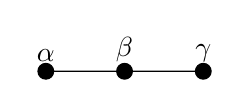
\begin{tikzpicture}
\draw[fill=black] 
(0,0) circle [radius=.1] node [above] {$\alpha$} --
(1,0) circle [radius=.1] node [above] {$\beta$} --
(2,0) circle [radius=.1] node [above] {$\gamma$};
\end{tikzpicture}.
  
For $m\geq 2$ define $G_m$ as the group presented by generators $\mathcal{X}_m$ and the following three families of relations:
\begin{align}
 \label{eq:am} \tag{$a_m$} x_{\alpha}(\xi) x_{\alpha}(\eta) & = x_{\alpha}(\xi+\eta),&  \xi,\eta\in B_d,\ d\leq m;&\\
 \label{eq:bm} \tag{$b_m$} [x_\alpha(\xi), x_{\alpha'}(\eta))] &  = 1, & \text{in the case $\alpha+\alpha'\not\in\Phi\cup\{0\}$,}\\
 \nonumber                                                     &       & \xi \in B_d,\ \eta \in B_e,\ d,e\leq m;\\
 \label{eq:cm} \tag{$c_m$} [x_\alpha(\xi), x_{\alpha'}(\eta)] & = x_{\alpha+\alpha'}(N_{\alpha,\alpha'}\xi\eta), & \text{in the case $\alpha+\alpha'\in \Phi$,}\\
 \nonumber                                                    &  & \xi \in B_d,\ \eta \in B_e,\ d, e, d+e \leq m.
 \end{align}
For $m=1$ define $G_1$ as the group presented by generators $\mathcal{X}_1$, 
three above families of relations $(a_1), (b_1), (c_1)$ and the following additional family:
\begin{align}  \label{eq:d1} \tag{$d_1$} [[x_{\alpha+\beta+\gamma}(\xi), x_{-\gamma}(\eta)], x_{\beta+\gamma}(\zeta) ] & = 1, 
 & \xi,\eta,\zeta\in B_1,\ \text{ $(\alpha, \beta, \gamma)$ is an $\rA_3$-triple. }
\end{align}

The obvious embedding of generators $\mathcal{X}_m \subseteq \mathcal{X}_{m+1}$ induces a map $f_m\colon G_m \to G_{m+1}$.
Our goal is to show the following result.
\begin{prop}\label{prop:tul3.3}
 For $m\geq 1$ the map $f_m$ is an isomorphism. Consequently, $\St(\Phi, B)$ can be presented by generators $\mathcal{X}_1$ and relations $(a_1)$, $(b_1)$, $(c_1)$, $(d_1)$.
\end{prop}
\begin{rem}
   Notice that for $\Phi=\rA_\ell$, $\ell\geq 4$ the group $\St(\Phi, B)$ admits a shorter presentation with family~ $(d_1)$ omitted (see~\cite[Lemma~3.3]{Tu83}).
   This is also true for $\Phi=\rE_\ell$ since $\St(\rE_\ell, R)$ can be presented as an amalgamated product of several copies of $\St(\rA_4, R)$, (cf. e.\,g.~\cite[Lemmas~3,7)]{S15}).   
  On the other hand, we believe that the above presentation is the shortest possible in the cases $\Phi=\rA_3, \rD_\ell$. \end{rem}

We will use the following commutator identities (cf.~\cite[H1]{Re75}):
\begin{align}
 \label{eq:H1ii}  [ab, c] = {}^a[b, c] \cdot [a,c];&\\ %= [a,[b,c]]\cdot [b,c] \cdot [a,c];&\\
 \label{eq:H1iii} [a,c]   = 1    \text{ implies } [a, [b,c]] = [[a,b],{}^bc].&
\end{align}

\begin{lemma}
 Suppose $m \geq 1$.
 Let $\alpha, \beta, \alpha', \beta' \in \Phi$ be such that $\alpha + \beta = \alpha' + \beta'$.
 Assume, moreover, that $\xi \in B_d$, $\xi' \in B_{d'}$, $\eta \in B_e$, $\eta' \in B_{e'}$ are such that 
  $N_{\alpha, \beta} \xi \eta = N_{\alpha', \beta'}\xi' \eta'$ for some $d,d',e,e'\leq m$ satisfying $d+e=d'+e' = m+1$.
 Then the following relations holds in $G_m$:
 \begin{equation}
  \label{eq:S-correctness} [x_\alpha(\xi), x_\beta(\eta)] = [x_{\alpha'}(\xi'), x_{\beta'}(\eta')].
 \end{equation}
 Moreover for every $\zeta \in B_{k''}$, $k''\leq m$ and $\gamma\in\{\alpha, \beta, \alpha + \beta\}$
  the following relation holds in $G_m$:
 \begin{equation}
 \label{eq:S-commutes} [[x_\gamma(\zeta), [x_\alpha(\xi), x_\beta(\eta)]] = 1.
 \end{equation}
\end{lemma}
\begin{proof}
 Notice that $k+l = m+1$, $k, l\leq m$ imply $k,l>0$, hence $B_i= A \cdot t^i$ for $i=k,k',l,'l'$.
 This means that without loss of generality we may assume that $\mathfrak{m}=0$ and $B = A[t]$.
 But now our statement is not different from~\cite[Proposition 1.1]{Re75} (or~\cite[Proposition~3.2.2]{RS76} in the case $g=1$)
  and can be proved by the same argument which remains valid for a general coeffient ring $A$.
\end{proof}

For every $\xi \in B_{m+1}$ and $\alpha\in \Phi$ there exist $\xi' \in B_m$ and $\alpha'\in \Phi$ such that $\xi = t\xi'$ and $\alpha-\alpha'\in\Phi$,
so we can define the following element of $G_m$:
\begin{equation} \label{eq:S-definition} S_\alpha(\xi) := [x_{\alpha-\alpha'}(N_{\alpha-\alpha',\alpha'} \xi'), x_{\alpha'}(t)].\end{equation} 
From~\eqref{eq:S-correctness} it follows that $S_\alpha(\xi)$ does not depend of the choice of $\alpha'$.

Let us show that elements $S_\alpha(\xi)$ satisfy the relations $(a_{m+1})$, $(b_{m+1})$ and $(c_{m+1})$.
From \eqref{eq:H1ii} and~\eqref{eq:S-commutes} it follows that $S_\alpha(\xi)$ satisfy $(a_{m+1})$ and hence $(b_{m+1})$ in the special case $\alpha=\alpha'$.
\begin{lemma} \label{lem:cm-plus1} Suppose that $m\geq 1$. For every $\alpha, \alpha' \in \Phi$ such that $\alpha+\alpha' \in \Phi$ and
 $a\in A$, $\xi \in B_d$, $d \leq 0$ the following relation holds in $G_m$: 
\begin{equation} \nonumber
[x_\alpha(\xi), S_{\alpha'}(at^{m+1})] = [x_\alpha(t\xi), x_{\alpha'}(at^m)] = S_{\alpha+\alpha'}(N_{\alpha,\alpha'}a\xi t^{m+1}).
\end{equation}
\end{lemma}
\begin{proof}
By \cite[Lemma~3.1.2]{RS76} we may assume without loss of generality that $\alpha'=\beta$ for some $\rA_3$-triple $(\alpha, \beta, \gamma)$.
\begin{align*}
   [x_\alpha(\xi), S_\beta(at^{m+1})] = [x_\alpha(\xi), [x_{\beta + \gamma}(t), x_{-\gamma}(a't^m)]]
   &  \text{ by~\eqref{eq:S-correctness},\eqref{eq:S-definition} for $a' = N_{\beta+\gamma, -\gamma} a$} \\ 
 = [x_{\alpha+\beta+\gamma}(\epsilon t\xi), {}^{x_{\beta+\gamma}(t)}x_{-\gamma}(a't^m)]             
 &  \text{ by~\eqref{eq:H1iii}, for $\epsilon=N_{\alpha, \beta+\gamma}$} \\
 = {}^{x_{\beta+\gamma}(t)}[x_{\alpha+\beta+\gamma}(\epsilon t\xi), x_{-\gamma}(a't^m)]             
 &  \text{ by $(b_1)$}
\end{align*} 
Denote by $R$ the expression in the right hand side of the above formula.
\begin{enumerate}
 \item \label{case:cm-1} Case $m=1$, $d = 0$.
 \begin{align*}
   R  = [x_{\alpha +\beta + \gamma}(\epsilon t\xi), x_{-\gamma}(a't)] 
   & \text{ by $(d_1)$}\\
      = {}^{x_{\beta+\gamma}(1)}[x_{\alpha +\beta + \gamma}(\epsilon t\xi), x_{-\gamma}(a't)] 
   & \text{ by~\eqref{eq:H1ii}, $(b_1)$, $(c_1)$} \\
      = [x_\alpha(\xi), [x_{\beta + \gamma}(1), x_{-\gamma}(a't^m)]] 
   & \text{ by $(b_1)$, \eqref{eq:H1iii}}\\
      = [x_\alpha(t\xi), x_\beta(at)]
   & \text{ by~\eqref{eq:S-correctness},\eqref{eq:S-definition}.}
 \end{align*}  
 \item \label{case:cm-2} Case $m\geq 2$ or $m=1$, $d < 0$.
 \begin{align*}
 R = {}^{x_{\beta+\gamma}(t)}[x_{\alpha+\beta+\gamma}(\epsilon t^2\xi), x_{-\gamma}(a't^{m-1})]     
 &  \text{ by~\eqref{eq:S-correctness} if $k=0$ or~\eqref{eq:cm} if $k <0$} \\
 = [[x_\alpha(t\xi), x_{\beta+\gamma}(t)], {}^{x_{\beta+\gamma}(t)} x_{-\gamma}(a't^{m-1})]         
 &  \text{ by~$(b_2)$, $(c_2)$ or by~\eqref{eq:S-commutes},\eqref{eq:S-definition} if $m=1$} \\
 = [x_\alpha(t\xi), x_\beta(at^m)]                                                                  
 &  \text{ by~\eqref{eq:H1iii}. \qedhere}
\end{align*} 

\end{enumerate}
\end{proof}

It will be convenient for us to extend the definition of $S_\alpha(\xi)$ by allowing $\xi$ to take values in $B_d$ for $d\leq m$.
In this case we simply set $S_\alpha(\xi) = x_\alpha(\xi)$.

Now suppose  $0 \leq d \leq m+1$. Clearly \eqref{eq:S-correctness} and \eqref{eq:S-definition} (in the case $1\leq d\leq m$) or~\cref{lem:cm-plus1} (in the case $d=0,m+1$) imply that
\begin{equation} \label{eq:cm-plus1-generalized} 
[S_\alpha(\xi), S_{\alpha'}(\eta)] = S_{\alpha+\alpha'}(N_{\alpha,\alpha'}\xi \eta),\ \xi \in B_d, \eta \in B_{m+1-d}.
\end{equation}

We need to introduce additional notation.
For $a,b\leq m+1$ we denote by $\bot(a, b)$ (resp. $\angle(a,b)$) the family of all relations $[S_\alpha(\xi), S_{\alpha'}(\eta)] = 1$
for which $\xi \in B_a$, $\eta \in B_b$ and $\alpha$ and $\alpha'$ are orthogonal (resp. form a sharp angle). 
We denote by $\bot_0(a, b)$ the subset of $\bot(a, b)$
consisting of those relations for which $\xi = t^{a} \in B_a$.

\begin{lemma} \label{claim1} In $G_m$ relations $\bot_0(1, d)$ and $\angle(d, m)$ imply $\angle(d, m+1)$ for $d\leq m+1$ \end{lemma}
\begin{proof}
Without loss of generality we may assume that $\alpha' = \alpha + \beta$
  for some $\rA_3$-triple $(\alpha, \beta, \gamma)$.
Write $\eta = bt^{m+1}$ for some $b\in A$.
\begin{align*} 
[S_\alpha(\xi), S_{\alpha+\beta}(bt^{m+1})] = [S_\alpha(\xi), [x_{\alpha+\beta+\gamma}(b't^m), x_{-\gamma}(t)]] & \text{ by~\eqref{eq:S-correctness} and~\eqref{eq:S-definition}}\\
= [[S_\alpha(\xi), x_{\alpha+\beta+\gamma}(b't^m)], {}^{x_{\alpha+\beta+\gamma}(b't^m)}\!x_{-\gamma}(t)] & \text{ by~$\bot_0(1, d)$}\\
= 1
 & \text{ by~$\angle(d, m)$. \qedhere} \end{align*} 
\end{proof}

\begin{lemma} \label{claim2} In $G_m$ relations $\angle(d, m+1)$ imply $\bot_0(d, m+1)$ for  $1\leq d\leq m+1$. \end{lemma}
\begin{proof}
As before, without loss of generality we may assume $\alpha' = \gamma$ for some $\mathsf{A}_3$-triple $(\alpha, \beta, \gamma)$.
 \begin{align*}
 {}^{S_\gamma(t^d)}S_\alpha(bt^{m+1}) = {}^{S_\gamma(t^d)}[S_{-\beta}(b't^{m+1}), x_{\alpha+\beta}(1)] & \text{ by~\cref{lem:cm-plus1}}\\
 = [S_{-\beta}(b't^{m+1}), {}^{S_\gamma(t^d)}x_{\alpha+\beta}(1)]                                     
 & \text{ by $\angle(d, m+1)$}\\
 = [[x_{-\beta-\gamma}(b''t^{m+1-d}), S_\gamma(t^d)], {}^{S_\gamma(t^d)}x_{\alpha+\beta}(1)]          
 & \text{ by~\eqref{eq:cm-plus1-generalized}}\\
 = [x_{-\beta-\gamma}(b''t^{m+1-d)}), [S_\gamma(t^d), x_{\alpha+\beta}(1)]]                           
 & \text{ by~\eqref{eq:H1iii} and $(b_{m+1-d})$}\\
 = S_{\alpha}(b'''t^{m+1})                                                                            
 & \text{ by~\eqref{eq:cm-plus1-generalized}.} \end{align*}
Usual identities for structure constants imply (cf.~\cite[p.~12]{Re75}):
 $b'''=N_{-\beta-\gamma, \alpha+\beta+\gamma} \cdot N_{\gamma, \alpha+\beta} \cdot N_{-\beta-\gamma, \gamma} \cdot N_{-\beta, \alpha+\beta} \cdot b = b,$ from which the claim follows.
\end{proof}

\begin{lemma} \label{claim3}
 In $G_m$ relations $\bot_0(d, m+1)$, $\angle(d, d)$ and $\angle(m+1, m+1)$ imply $\bot(d, m+1)$ for $d\leq m+1$.
\end{lemma}
\begin{proof}
 \begin{align*} 
 S_{\alpha+\beta+\gamma}(abt^{m+1}) = {}^{S_{-\beta}(t^d)}\!S_{\alpha+\beta+\gamma}(abt^{m+1}) 
 & \text{ by $\bot_0(d, m+1)$}\\
 = {}^{S_{-\beta}(t^d)}\![x_{\alpha+\beta}(b't^{m+1-d}), S_\gamma(at^d)] 
 & \text{ by~\eqref{eq:cm-plus1-generalized}} \\
 = [S_{\alpha}(b't^{m+1}) x_{\alpha+\beta}(b't^{m+1-d}), S_\gamma(at^d)] 
 & \text{ by~\eqref{eq:cm-plus1-generalized} and $\angle(d, d)$ }\\
 = {}^{S_{\alpha}(b't^{m+1})}\!S_{\alpha+\beta+\gamma}(abt^{m+1}) [S_{\alpha}(b't^{m+1}), S_\gamma(at^d)] 
 & \text{ by~\eqref{eq:H1ii} and~\eqref{eq:cm-plus1-generalized}} \\
 = S_{\alpha+\beta+\gamma}(abt^{m+1}) [S_{\alpha}(b't^{m+1}), S_\gamma(at^d)] 
 & \text{ by $\angle(m+1, m+1)$. \qedhere}
\end{align*}
\end{proof}

\begin{lemma} \label{lem:bm-plus1}
Elements $S_\alpha(\xi)$ satisfy relations $(b_{m+1})$.
 \end{lemma}
\begin{proof}
We must show that $S_\alpha(\xi)$ satisfy $\angle(d, m+1)$ and $\bot(d, m+1)$ for $d\leq m+1$.
\begin{enumerate}
 \item Relations $\angle(d, m+1)$, $d\leq m$ follow from~\cref{claim1}. 
 \item Relations $\bot(d, m+1)$ with $d\leq 0$ can verified by direct computation:
 \begin{align*} 
 [x_\alpha(\xi), S_{\gamma}(bt^{m+1})] = [x_\alpha(\xi), [x_{\beta+\gamma}(b't^m), x_{-\beta}(t)]] & \text{ by~\eqref{eq:S-correctness},\eqref{eq:S-definition}} \\
 = [[x_\alpha(\xi), x_{\beta+\gamma}(b't^m)], {}^{x_{\beta+\gamma}(b't^m)}\!x_{-\beta}(t)] &
 \text{ by \eqref{eq:H1iii} and $(b_1)$} \\
 = {}^{x_{\beta+\gamma}(b't^m)}\![x_{\alpha+\beta+\gamma}(b't^m\xi), x_{-\beta}(t)] &
 \text{ by $(b_m)$ and $(c_m)$} \\
 = 1 & \text{ by $(b_m)$.}
\end{align*}
 \item Relations $\bot_0(d, m+1)$ with $1\leq d\leq m$ follow from~\cref{claim2}.
 \item Relations $\angle(m+1, m+1)$ follow from~\cref{claim1}, consequently relations $\bot_0(m+1, m+1)$ follow from~\cref{claim2}.
 \item Relations $\bot(d, m+1)$, $0\leq d\leq m+1$ follow from~\cref{claim3} and the previous two assertions.
\end{enumerate}
\end{proof}

\begin{proof}[Proof of~\cref{prop:tul3.3}]
Define the map $g_m\colon G_{m+1} \to G_m$ by $g_m(x_\alpha(\xi)) = S_\alpha(\xi)$.
In view of the above lemmata this map is well-defined. It is clear that $g_m$ is inverse to $f_m$, which proves the first claim.

Denote by $G_\infty$ the group presented by generators $\mathcal{X}_\infty$ and relations $(a_\infty)$, $(b_\infty)$, $(c_\infty)$.
By the above argument there is an isomorphism between $G_1$ and $\colim\limits_{n\to\infty} G_n \cong G_\infty$.

Denote by $i\colon G_\infty \to \St(\Phi, B)$ the map induced by the obvious embedding of $\mathcal{X}_\infty$ into the set of 
 Steinberg generators of $\St(\Phi, B)$.  
Using~\eqref{eq:H1ii} multiple times it is not hard to show that the map $j\colon \St(\Phi, B) \to G_\infty$ given by
 $j(x_\alpha(b)) = \prod x_\alpha(b_i)$, where $b = \sum b_k$ is the decomposition of $b$ into a finite sum of its homogeneous components $b_k\in B_k$, is a well-defined map.
It is clear that $i$ and $j$ are mutually inverse. 
\end{proof}

\end{comment}

\printbibliography

\end{document}
